\documentclass[12pt]{report}
\usepackage{mathptmx}
\usepackage[margin=0.7in,right=1in,left=1.5in]{geometry}
\usepackage{graphicx}
\usepackage{setspace}
\usepackage{mathtools}
\usepackage{amsmath}
\usepackage[section]{placeins}
\usepackage{multicol}
\usepackage{acronym}
\usepackage{array}
\usepackage{array}
\usepackage[pscoord]{eso-pic}
\renewcommand\bibname{References}
\newcolumntype{P}[1]{>{\centering\arraybackslash}p{#1}}
\newcolumntype{M}[1]{>{\centering\arraybackslash}m{#1}}
\renewcommand{\baselinestretch}{1} 

%\singlespacing
\linespread{1.25}

\begin{document}
	\begin{titlepage}
		\begin{center}
			\LARGE {\bfseries {ESTIMATION OF OPTICAL SIGNAL TO NOISE RATIO USING NEURAL NETWORK}}\\
			\vspace{1.5cm}
			{\normalsize 
			\textbf{Md.Asadouzzaman}\\
			Student \# 142067\\
			\textbf{Dulal Hossain}\\
			Student \# 142090\\
			\textbf{Abdul Motin}\\
			Student \# 142062\\}
		\vspace{5cm}
			\centering{
\includegraphics[scale=0.3]{figure/duet_logo.png}}\\
			\vspace{4cm}
			{\fontsize{13}{0} \bfseries {DHAKA UNIVERSITY OF ENGINEERING \& TECHNOLOGY, GAZIPUR}}
			{\fontsize{12}{0} \bfseries {DEPARTMENT OF ELECTRICAL AND ELECTRONIC ENGINEERING}}\\
			{\fontsize{12}{0} \textbf{July, 2019}}
		\end{center}
	\end{titlepage}
	\begin{titlepage}
		\begin{center}
			\LARGE {\bfseries {ESTIMATION OF OPTICAL SIGNAL TO NOISE RATIO USING NEURAL NETWORK}}\\
			\vspace{6cm}
			{\normalsize 
				\textbf{Md.Asadouzzaman}\\
				Student \# 142067\\
				\textbf{Dulal Hossain}\\
				Student \# 142090\\
				\textbf{Abdul Motin}\\
				Student \# 142062\\}
			\vspace{9cm}
			{\fontsize{12}{0} \bfseries {DEPARTMENT OF ELECTRICAL AND ELECTRONIC ENGINEERING}}
			{\fontsize{13}{0} \bfseries {DHAKA UNIVERSITY OF ENGINEERING \& TECHNOLOGY, GAZIPUR}}\\
			{\fontsize{12}{0} \textbf{July, 2019}}
		\end{center}
	\end{titlepage}
	\begin{titlepage}
	\begin{center}
		\LARGE {\bfseries {ESTIMATION OF OPTICAL SIGNAL TO NOISE RATIO USING NEURAL NETWORK}}\\
		\vspace{1cm}
		{\fontsize{12}{0} \bfseries {A THESIS}}\\
		
		{\normalsize  {Submitted in partial fulfillment of the requirements for the award of the degree\\of}}
		
		{\fontsize{12}{0} \bfseries {BACHELOR OF SCIENCE}}\\
		{\fontsize{12}{0} \bfseries {IN}}\\
		{\fontsize{12}{0} \bfseries {ELECTRICAL AND ELECTRONIC ENGINEERING}}\\
		{\fontsize{12}{0} \bfseries {By}}\\
		
		{\normalsize 
		\textbf{Md.Asadouzzaman}\\
		Student \# 142067\\
		Registration\# \\
		Session 2017-2018\\}
		\begin{multicols}{2}
			\normalsize 
				\textbf{Dulal Hossain}\\
				Student \# 142090\\
				Registration\# \\
				Session 2017-2018\\
				\textbf{Abdul Motin}\\
				Student \# 142062\\
				Registration\# \\
				Session 2017-2018\\
		\end{multicols}
		\vspace{1cm}
		{\normalsize 
			Under supervision of\\\vspace{1cm}
			\rule{5cm}{.1cm}\\
			\textbf Dr. Md. Saifuddin Faruk\\
			Professor\\}
		\vspace{0.5cm}
		{\fontsize{12}{0} \bfseries {DEPARTMENT OF ELECTRICAL AND ELECTRONIC ENGINEERING}}
		{\fontsize{13}{0} \bfseries {DHAKA UNIVERSITY OF ENGINEERING \& TECHNOLOGY, GAZIPUR}}\\
		{\fontsize{12}{0} \textbf{July, 2019}}
	\end{center}
\end{titlepage}

\begin{center}
	\section*{ACKNOWLEDGMENT}
	\pagenumbering{roman}
\end{center}
	We would like to express our deepest appreciation to all those who provided us the possibility to complete this thesis.  A special gratitude we give to our final year thesis  supervisor, Dr. Md. Saifuddin Faruk, Professor, Dept. of EEE, DUET, whose contribution in stimulating suggestions and encouragement,  helped us to coordinate our thesis. We also place on record, our sense of gratitude to one and all, who directly or indirectly, have lent their hand in this venture.\\ [1cm]

		\begin{minipage}[t]{0.3\textwidth}
			\begin{flushleft}
				DUET, Gazipur\\
				Bangladesh\\
				September, 2019
			\end{flushleft}
		\end{minipage}
	\begin{minipage}[t]{0.65\textwidth}
		\begin{flushright}
			Author\\
			Md. Asadouzzaman\\
			Abdul Motin\\
			Dulal Hossain
		\end{flushright}
	\end{minipage}
	
	\pagebreak
%\begin{center}
	\section*{ABSTRACT}
	The quality of the optical signal is generally assessed by means of optical-signal-to-noise ratio (OSNR) which is defined as the ratio of the signal power and the ASE noise power in a reference bandwidth. OSNR is one of the key parameters for optical performance monitoring which enables fault management of optical transmission systems and networks including diagnosis and localization.
	
	There are several methods of optical signal to noise ratio estimation. Second and fourth order moments method is one of them. This paper aims to investigate the performance of conventional $M_2M_4$ methods and find a way to overcome the limitation of this method. We propose a novel method of optical signal to noise ratio using a digital coherent receiver, where OSNR is determined from second and fourth order statistical moments of equalized signals in any modulation format. A modification in second and fourth order moment structure to perform better on the channel of interest is of our aim. This method shows better performance for 4-QAM (Quadrature Amplitude Modulation) and shows a high error in estimation of high OSNR. To solve this problem for higher QAM an algorithm is developed. In proposed method, a fully connected feedforward neural network is trained using two information extracted from constellation diagram. One is second order momentum of all symbol another one is variance in absolute value of second ring to estimate OSNR estimator structures for both real and complex channels are examine as well as simulation is performed for both AWGN (Additive White Gaussian Noise) added and for practical long haul communication. For certain value of OSNR second and fourth order moments method is suitable for OSNR estimation whereas our proposed method is suitable for high OSNR estimation.Effectiveness of the proposed method is validated with computer simulation for 16-QAM and 64-QAM. 
%\end{center}

	\listoffigures
	\pagebreak
\begin{center}
	\section*{ACRONYMS}
\end{center}
\begin{acronym}
	\acro{QAM}{Quadrature Amplitude Modulation}
	\acro{QPSK}{Quadrature Phase Shift Keying}
	\acro{OSNR}{Optical Signal to Noise Ratio}
	\acro{ANN}{Artificial Neural Network}
	\acro{DNN}{Deep Neural Network}
	\acro{AWGN}{Additive White Gaussian Noise}
	\acro{WDM}{Wavelength Division Multiplexed}
	\acro{DSP}{Digital Signal Processing}
	\acro{DFB}{Distributed Feedback Laser}
	\acro{SMF}{Single Mode Fiber}
	
\end{acronym}
	\tableofcontents
	
	
	
	
	
	\chapter{INTRODUCTION}
	\pagenumbering{arabic}
	\section{Introduction}
	The search for a good signal -to- noise ratio (SNR) estimation technique is motivated by the fact that various algorithms require knowledge of the SNR for optimal performance if the SNR is not constant.Therefore, it is important to estimate optical signal to noise ratio (OSNR) which is basically the ratio of optical signal and ASE noise over a reference bandwidth, in order to get a real-time information of signal health in an optical network \cite{OPMTech}. The performance of diverse systems may be improved if knowledge of the SNR is available. 
	
	Past engineering practice has often used estimation of the total signal plus noise power instead of estimation of the SNR, since it is much easier to measure total power than the ratio of signal power to noise power. However, decreasing hardware costs and increasing demands for pushing system performance to the achievable limits make an investigation of SNR estimation techniques timely. 
	There are several methods of optical signal to noise ratio estimation. One of the common method is second and fourth order moment calculation method. In this research, we attempt to improve the current method for higher order QAM. Practical investigation shows that second and fourth order moment method is appropriate for lower order QAM for the purpose of SNR monitoring. But for higher order QAM when the SNR is varying to a higher value it cannot estimate it properly. To solve this problem an attempt is taken in this literature.

	The estimation result of second and fourth order moment method shows good result for QPSK and 4-QAM. Instead of taking all the signals from the constellation diagram, only taking certain number of signal from the constellation diagram of 16-QAM, 32-QAM, 64-QAM, 128-QAM and 256-QAM, we can solve the problem. 
	
	The estimator under consideration derive the SNR from the baseband, sampled, data-bearing received signal. The data may be known or unknown to the receiver. Those technique which derive the SNR estimates solely from the unknown, information-bearing portion of the received signal are known as “in-service” SNR estimators and are of particular interest since they do not impinge upon the through out of the channel.

	\section{Objectives }
	\begin{enumerate}
		\item  To investigate the performance of conventional second and fourth order moment method.
		\item  To develop an algorithm to improve the performance of conventional second and fourth order moment method.
	\end{enumerate}
	\section{Literature Review} 
	A quite number of OSNR monitoring technique is developed for satisfactory OSNR monitoring. A deep neural networks (DNN) based OSNR monitoring technique is developed by Takahitu Tanimura and Jens Rasmussen \cite{deepOSNR}.They demonstrate a use of deep neural networks (DNN) for OSNR monitoring with minimum prior knowledge. By using 5-layers DNN trained with 400,000 samples, the DNN successfully estimates OSNR in a 16-GB DP-QPSK system. 
	
	The study is performed using principal component analysis-based pattern recognition on asynchronous delay-tap plots and it yields accurate results in the simultaneous monitoring of linear impairments. Another recent work facing the limited scalability, which are based on the prior knowledge of a determined set of signals, where a deep neural network (DNN), trained with raw data asynchronously sampled by a coherent receiver is proposed for OSNR monitoring.
	
	In a digital coherent optical receiver OSNR estimation can be realized as a by-product of DSP algorithms. Several methods such as error vector magnitude(EVM) \cite{errorVector}, amplitude noise correlation \cite{nonlin}, Stokes parameter \cite{densityDistributions}, Gaussian process regression \cite{Gaussian} based methods have been investigated, for coherent reception based OSNR monitoring including second and fourth order statistical moment ($M_2M_4$) \cite{inband,eqpsk}, where  OSNR is determined from second and fourth order statistical moments of equalized signals in any modulation format. Their proposed method is especially important in recently-developed Nyquist wavelength-division multiplexed (WDM) systems and$/$or re-configurable optical-add$/$drop-multiplexed (ROADM) networks, because in these systems and networks, we cannot apply the conventional OSNR estimation methods best on optical-spectrum measurement of the in band signal and the out of band noise .Effectiveness of the proposed method is validated with computer simulations of nyquist-WDM systems and ROADM networks using 25-Gbaud quadrature phase shift keying (QPSK) and 16-QAM formats.
	
	The performance of several signal-to-noise ratio (SNR) estimation techniques reported in a literature by David R. Pauluzzi and Norman C. Beaulieu \cite{compare}, are compared to identify the “best” estimator. The SNR estimators are investigated by the computer simulation of baseband signals in real Additive White Gaussian Noise (AWGN) and baseband 8-PSK signals in complex AWGN. The mean square error is used as a measure of performance. In addition to comparing the relative performances, the absolute levels of performance are also established; the simulation performances are compared to a published Cramer-Rao bound (CRB) for real AWGN and a CRB for complex AWGN that is derived there. Some known estimator structures are modified to perform better on the channel of interest. Estimator structures for both real and complex channels are examined. 
	As optical fiber communication has become very popular nowadays, OSNR monitoring has become a must at the receiver side. A vast scope of development is available in this field.
	\iffalse
	\section{Conclusion}
	\fi
	
	\chapter{BACKGROUND THEORY}
	\iffalse
	\section{Introduction}
	The optical fiber communication is the communication in which signal is transmitted or received through the fiber where the communicating frequency are converted into light in optical form by optical source i.e. LED, LASER with the velocity of light propagates through the fiber.
	\fi
	\section{History of Optical Fiber Communication}
	1880- Alexander Graham Bell repeated the x-on of speech using a light beam.\\
	1954- Harold Hopkins and Narinder Singh Kapany showed that rolled fiber glass allowed light to be transmitted. Initially it was considered that the light can traverse in only straight medium.\\
	1960- With inventor of the study LASER an intense coherent light source operating at just one wave length mode available by T.H. Maimon.\\ 
	1963- B. Urdles of several hundred glass fibers were used for small scale illumination. The attenuation of this fiber is greater than 100dB/km. So their use as X-on medium for optical communication was not considered.\\ 
	1966- C.K.Kad \& Hockman postulated the use of glass fibers as optical communication wave guides. The cause of high attenuation is intrinsic \& extrinsic loss. The glass fiber attenuation had to be reduced in less 20 dB/km.\\ 
	1970-works at the coring glass works produced a fiber with the required attenuation. After improves attenuation. Now the attenuation is 0.1 dB/km.
	\section{Basic Block Diagram of Optical Fiber}
	\begin{figure}[htbp]
		\centering{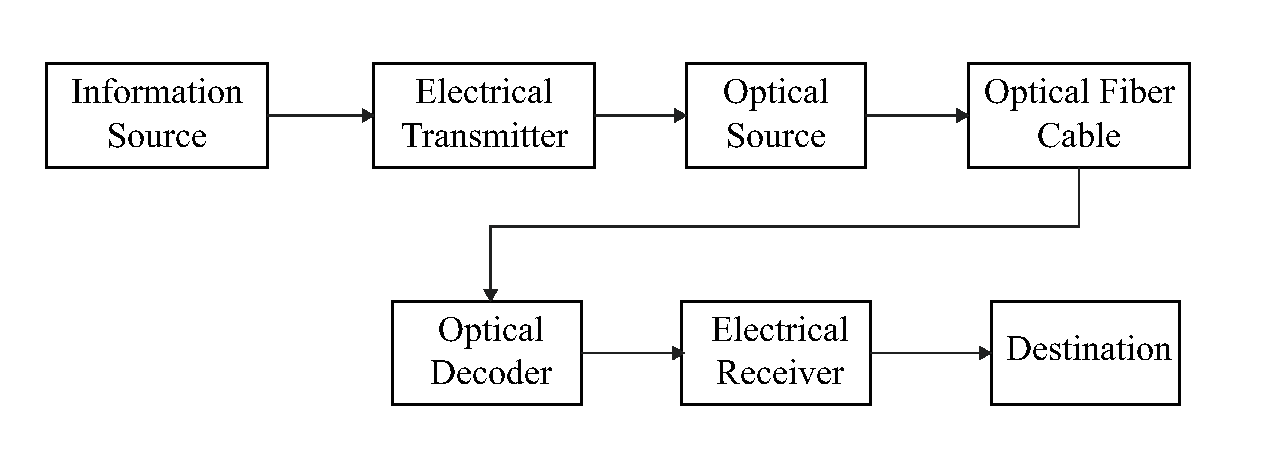
\includegraphics[scale=0.7]{figure/Optical+Fiber+Communications.eps}}
		\caption{Basic block diagram of optical fiber communication}
		\label{fig:block}
	\end{figure}
	
	Figure \ref{fig:block} shows basic block diagram of optical fiber communication. In this case the information source provides an electrical signal to a transmitter comprising an electrical stage which drives an optical source to give modulation of the light wave carrier. The optical source which provides the electrical–optical conversion may be either a semiconductor laser or light-emitting diode (LED). The transmission medium consists of an optical fiber cable and the receiver consists of an optical detector which drives a further electrical stage and hence provides demodulation of the optical carrier. Photo diodes (p–n, p–i–n or avalanche) and, in some instances, photo transistors and photo conductors are utilized for the detection of the optical signal and the optical–electrical conversion. Thus there is a requirement for electrical interfacing at either end of the optical link and at present the signal processing is usually performed electrically. The optical carrier may be modulated using either an analog or digital information signal. In the system shown in Figure \ref{fig:block} analog modulation involves the variation of the light emitted from the optical source in a continuous manner. With digital modulation, however, discrete changes in the light intensity are obtained (i.e. on–off pulses). Although often simpler to implement, analog modulation with an optical fiber communication system is less efficient, requiring a far higher signal-to-noise ratio at the receiver than digital modulation. Also, the linearity needed for analog modulation is not always provided by semiconductor optical sources, especially at high modulation frequencies. For these reasons, analog optical fiber communication links are generally limited to shorter distances and lower bandwidth operation than digital links.
	\section{Advantage of Optical Fiber Communication }
	\begin{enumerate}
			\item Enormous potential band width 
			\item  Small size and weight 
			\item  Electrical isolation 
			\item  Immunity to interference and cross talk 
			\item  Signal security 
			\item  Low transmission loss 
			\item  Ruggedness and flexibility 
			\item  System reliability and ease of maintenance 
			\item  Potential low cost
	\end{enumerate}
 
	\section{Construction of Optical Fiber}
	\begin{figure}[htbp]
		\centering{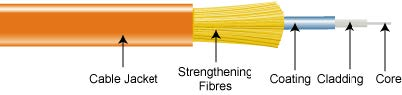
\includegraphics[scale=0.8]{figure/of_cable.jpg}}
		\caption{Basic construction of optical fiber}
		\label{fig:of_cable}
	\end{figure}
	\subsection*{Core}
	This is the physical medium that transports optical data signals from an attached light source to a receiving device. The core is a single continuous strand of glass or plastic that’s measured in microns ($\mu$) by the size of its outer diameter. The larger the core, the more light the cable can carry. All fiber optic cable is sized according to its core’s outer diameter. The three multimode sizes most commonly available are 50, 62.5, and 100 microns. Single-mode cores are generally less than 9 microns.
	\subsection*{Cladding}
	This is the thin layer that surrounds the fibre core and serves as a boundary that contains the light waves and causes the refraction, enabling data to travel throughout the length of the fibre segment. 
	\subsection*{Coating}
	This is a layer of plastic that surrounds the core and cladding to reinforce and protect the fibre core. Coatings are measured in microns and can range from 250 to 900 microns
	\subsection*{ Strengthening fiber } 
	These components help protect the core against crushing forces and excessive tension during installation. The materials can range from Kevlar® to wire strands to gel-filled sleeves. 
	\subsection*{Cable jacket}
	This is the outer layer of any cable. Most fibre optic cables have an orange jacket, although some types can have black or yellow jackets
	\section{Ray Transmission Theory}
		\begin{figure}[htbp]
		\centering{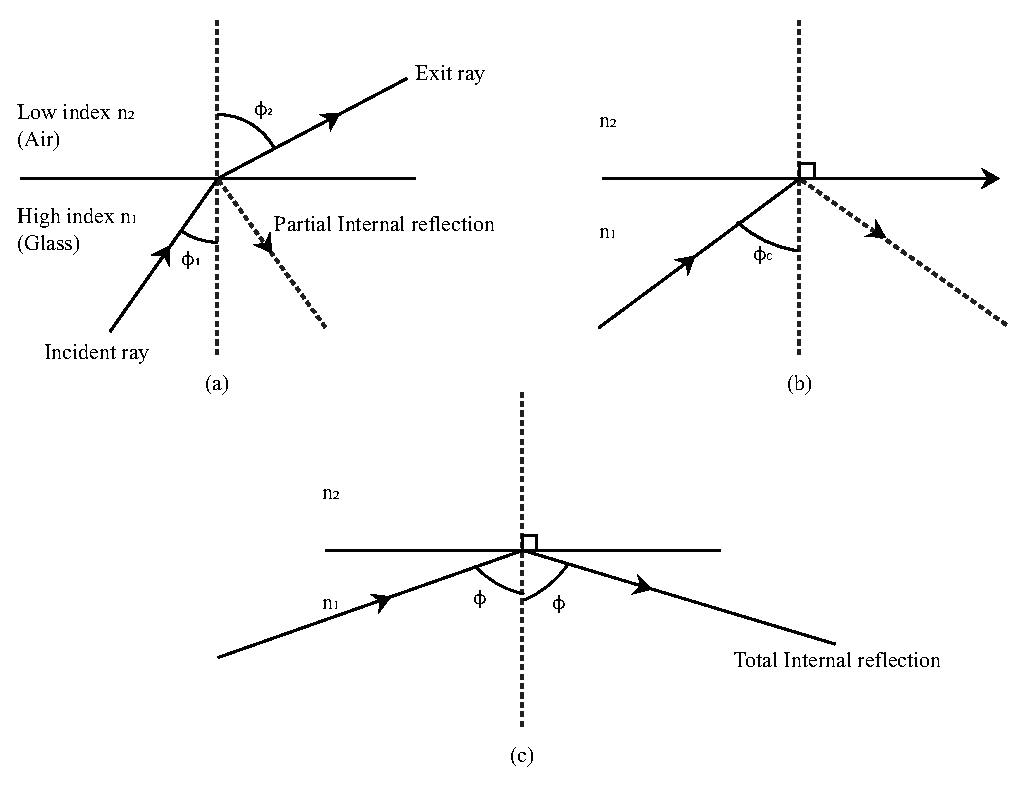
\includegraphics[scale=0.7]{figure/refraction.eps}}
		\caption{Light ray incident on a high to low refractive index interface (e.g glass air): (a) refraction; (b) the limiting case of refraction showing the critical ray at and angle $\phi_c$ (c) total internal reflection where $\phi > \phi_c$}
		\label{fig1}
	\end{figure}
The propagation of light within an optical fiber utilizing the ray theory model it is necessary to take account of the refractive index of the dielectric medium. The refractive index of a medium is defined as the ratio of the velocity of light in a vacuum to the velocity of light in the medium. A ray of light travels more slowly in an optically dense medium than in one that is less dense, and the refractive index gives a measure of this effect. When a ray is incident on the interface between two dielectrics of differing refractive indices. It may be observed that the ray approaching the interface is propagating in a dielectric of refractive index $n_1$ and is at an angle $\phi_1$ to the normal at the surface of the interface. If the dielectric on the other side of the interface has a refractive index $n_2$ which is less than $n_1$, then the refraction is such that the ray path in this lower index medium is at an angle $\phi_2$ to the normal, where $\phi_2$  is greater than $\phi_1$. The angles of incidence $\phi_1$ and refraction $\phi_2$ are related to each other and to the refractive indices of the dielectrics by Snell’s law of refraction which states that,
\begin{center}
	$n_1 Sin \phi_1 = n_2 Sin \phi_2$
\end{center}



	\section{Some Important Terms in Optical Fiber Communication }
	\subsection{ Acceptance Angle}
	The maximum angle to the axis at which light may enter the fiber in order to be propagated is called acceptance angle. 
	Any rays which are incident into the fiber core at an angle greater than $\alpha$ will be transmitted to core-cladding interface at an angle less than $\theta_c$,and will be totally internally reflected. 
	In Figure \ref{fig:of_propagation} the incident ray B at an angle then $\alpha$ is refracted into the cladding and loss by radiation
	\begin{figure}[htbp]
		\centering{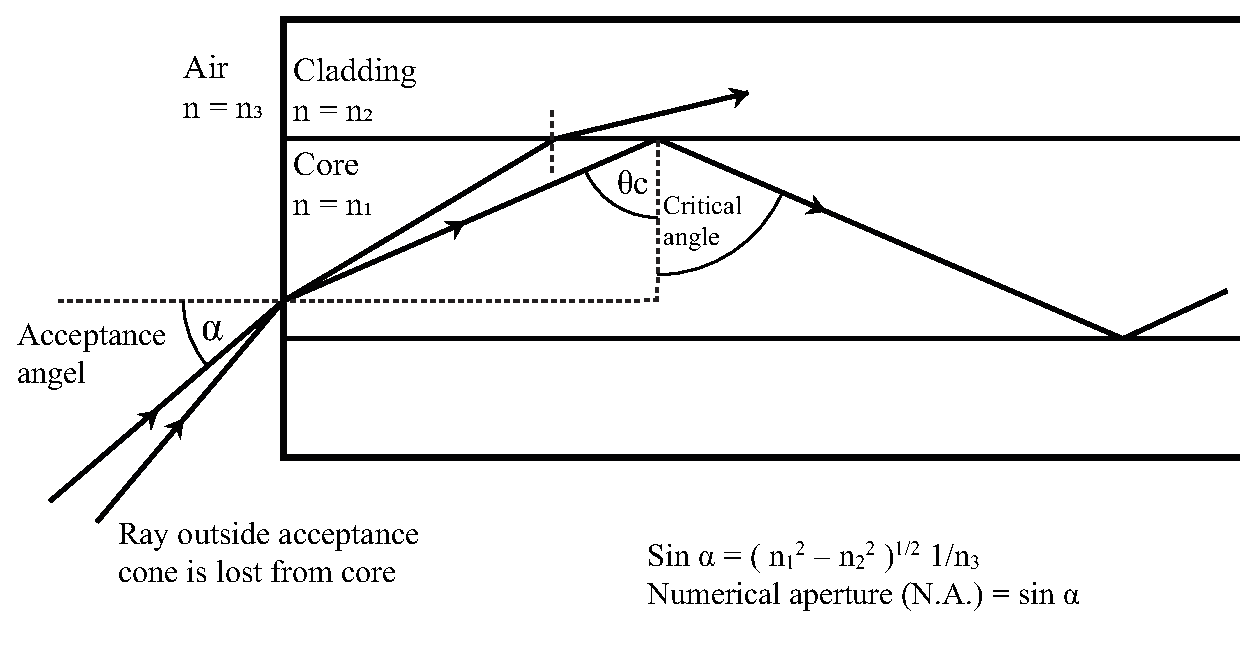
\includegraphics[scale=0.6]{figure/of_propagation.eps}}
		\caption{Launching light into an optical fiber}
		\label{fig:of_propagation}
	\end{figure}
	
	\subsection{Numerical aperture }
	In optics, the numerical aperture (NA) of an optical system is a dimensionless number that characterizes the range of angles over which the system can accept or emit light. By incorporating index of refraction in its definition, NA has the property that it is constant for a beam as it goes from one material to another, provided there is no refractive power at the interface. The exact definition of the term varies slightly between different areas of optics. Numerical aperture is commonly used in microscopy to describe the acceptance cone of an objective (and hence its light-gathering ability and resolution), and in fiber optics, in which it describes the range of angles within which light that is incident on the fiber will be transmitted along it. 
	
	
	\section{Attenuation}
	Every transmission line introduce some loss of signal power which is known is attenuation. Attenuation is the decrease in light power during light propagation along an optical fiber. Attenuation or Loss caused by violation of the condition of total internal reflection when launching light into a fiber. But practically speaking, fiber optic communications technology never considers this loss as a component of total attenuation because, without total internal reflection optical fiber simply does not work as a communication conduit. Attenuation can be categorized into three types- 
	\begin{figure}[htbp]
		\centering{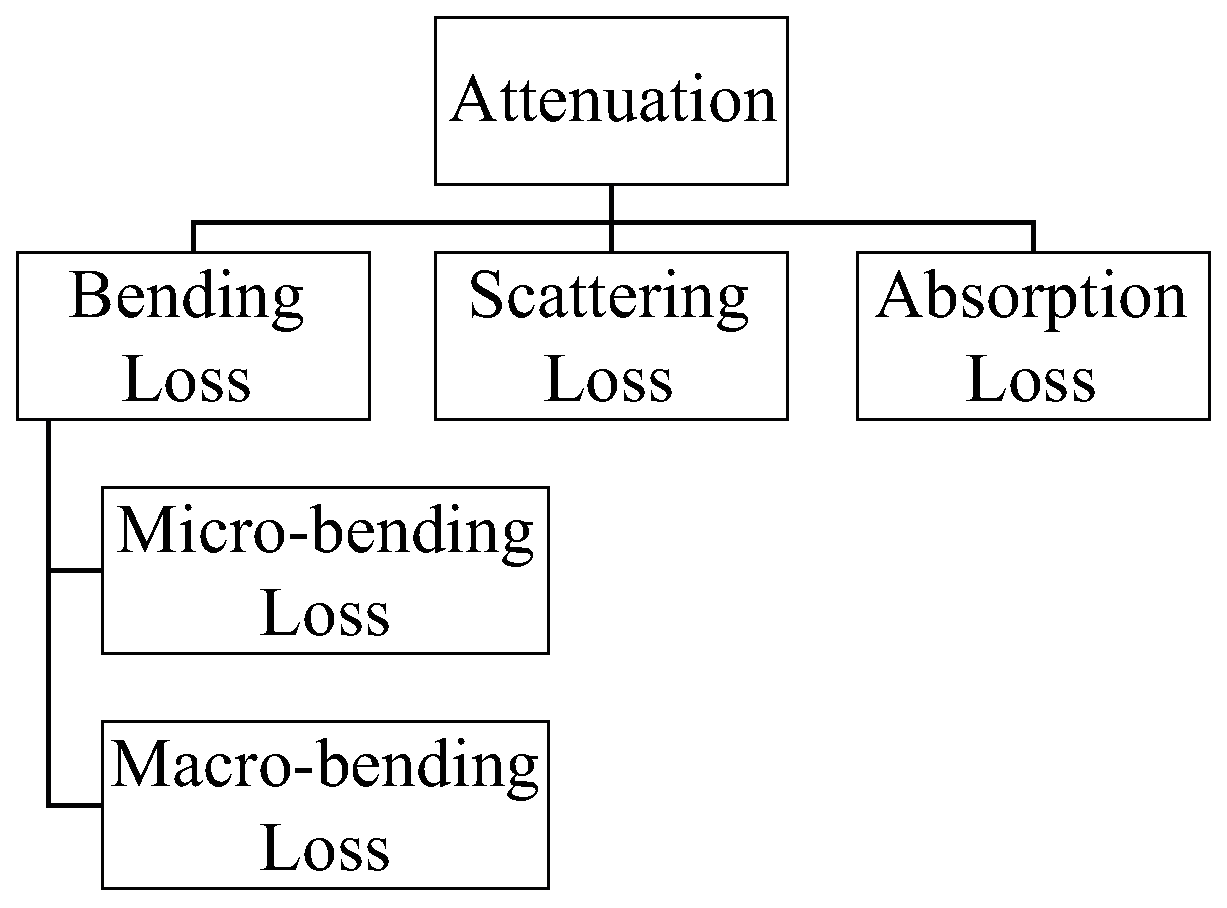
\includegraphics[scale=0.4]{figure/attenuation.eps}}
		\caption{Different types of attenuation.}
		\label{fig:attenuation}
	\end{figure}
	\subsection{Bending loss}
	There are two types of bending loss occurring in the optical fiber which fails to achieve total internal reflection. 
	
		\subsubsection{Micro-bending Loss}
	Micro-bending losses are caused by small imperfections in the fiber core. It is caused by manufacturing process. When the light beam meets these imperfections, changes its direction. The light beam which travel initially at the critical propagation angle, at this point it will be reflected and will change the angle of propagation. The result is that the condition of total internal reflection is not attained and portion of the beam will be refracted. As a result some portion of light lost in the fiber during propagation shown in figure \ref{fig:micro_benidng}.
	\begin{figure}[htbp]
		\centering{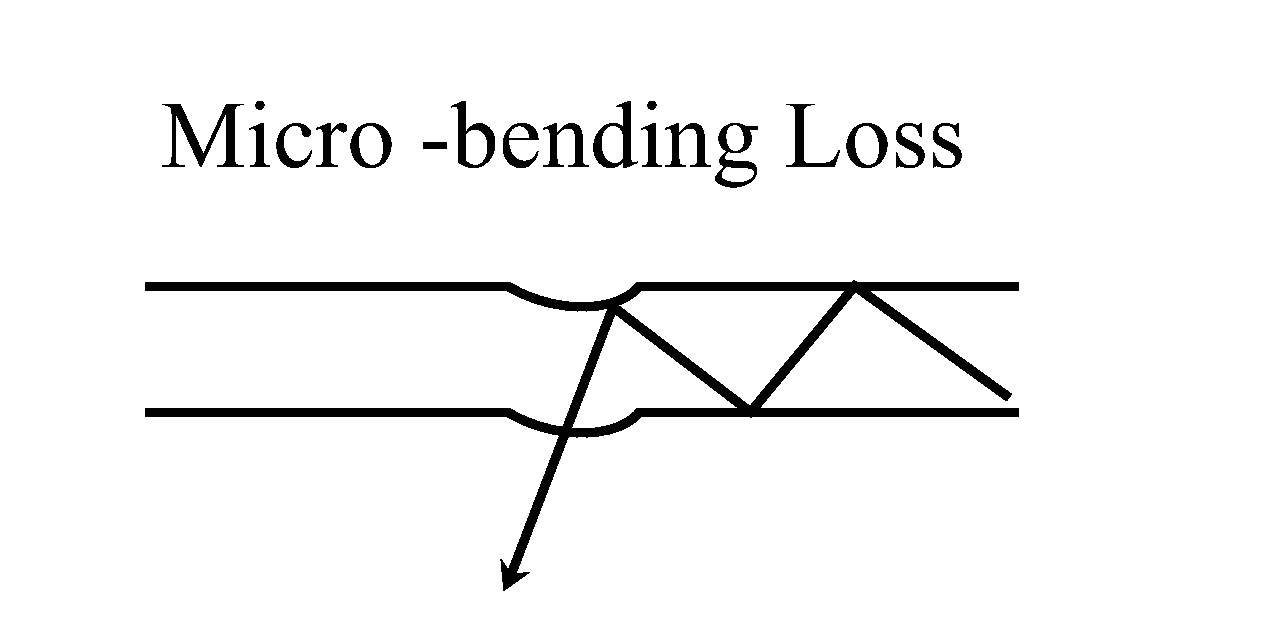
\includegraphics[scale=0.3]{figure/micro_bending.eps}}
		\caption{Macro-bending loss in optical fiber.}
		\label{fig:micro_benidng}
	\end{figure}

	\subsubsection{Macro-bending loss}
	Macro-bending happens when the fiber is bend into a large radius of curvature relative to the fiber diameter (large bends).These bends becomes a great source of power loss when the radius of curvature is less than several centimeters. At the bending point the incidence angle is smaller than critical angle for which some portion of the light ray is refracted. The result is failure to achieve total internal reflection in the bend fiber. Hence the power of the light arriving at its destination will be less than the power of the light emitted into the fiber from a light source. The propagation of light of a straight fiber and a bend fiber is shown in the figure \ref{fig:macro-bending}. 
	\begin{figure}[htbp]
		\centering{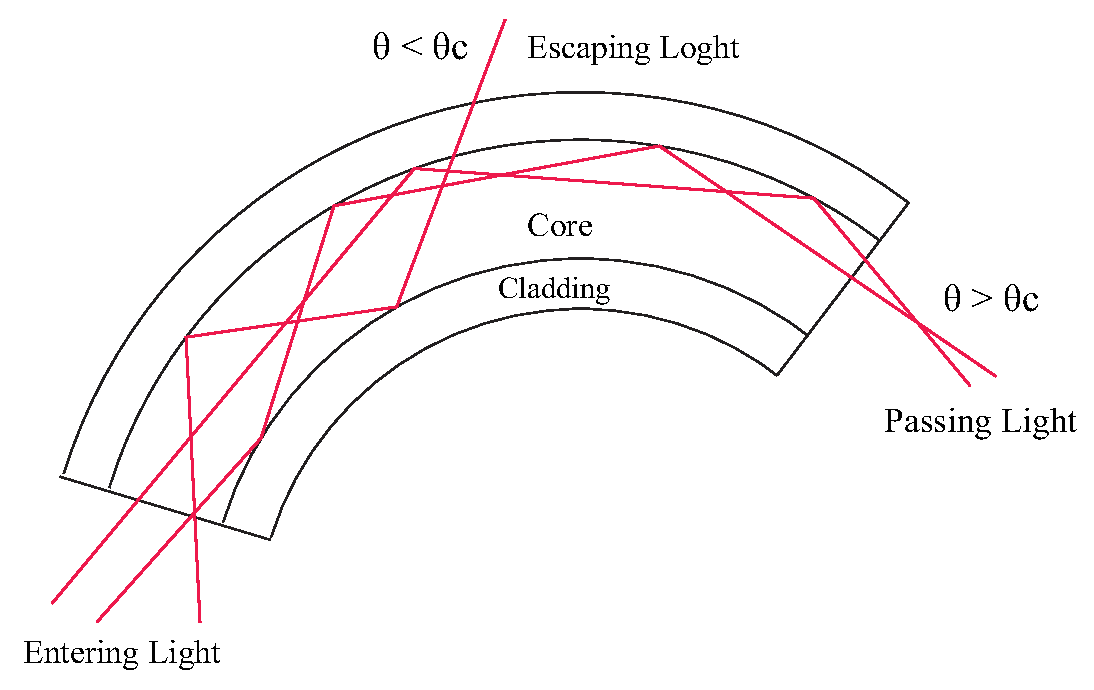
\includegraphics[scale=0.5]{figure/macro_bending.eps}}
		\caption{Macro-bending loss in optical fiber.}
		\label{fig:macro-bending}
	\end{figure}
	

	
	\subsection{ Scattering loss}
	The propagation of a light is based on total internal reflection of light wave. Rough and irregular surfaces can cause light ray to be reflected in random direction. Scattering losses occurs when a wave interacts with a particle in a way that removes in the directional propagating wave and transfers it to other directions. The light is note absorb, just send in another direction. There are two main types of scattering.\\ 
	\begin{itemize}
		\item Linear Scattering.
		\item Nonlinear Scattering.\\
	\end{itemize}

	For linear scattering, the amount of light power that is transferred from a wave is proportional to the power in the wave. It is characterized by heavy no change in frequency in the scattered wave. On the other hand, nonlinear scattering is accompanied by a frequency shift of the scatter light. Nonlinear scattering is caused by high values of electric field within the fiber (modest to high amount of optical power). Nonlinear scattering cause significant power to be scattered in the forward, backward, or sideways directions
	
		\begin{figure}[htbp]
		\centering{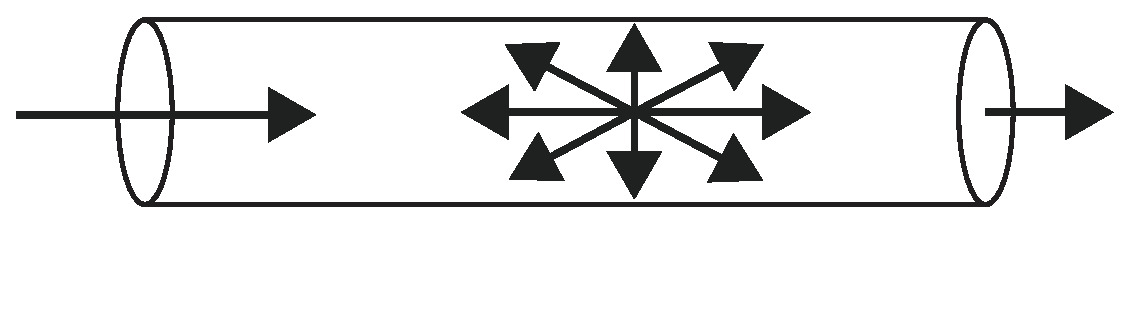
\includegraphics[scale=0.4]{figure/scattering.eps}}
		\caption{Scattering loss in fiber Optic}
		\label{fig:scttering_loss}
	\end{figure}
	\subsection{Absorption loss}
	If an incoming photon has such a frequency that its energy ($E_p=hf$) is equal to the energy gap ($\bigtriangleup$E) of the material, this photon will be absorbed by the material. $\bigtriangleup$E is the energy difference between the two energy levels. Light travels down an optical fiber and encounter a material whose energy level gap is exactly equal to the energy of this photons. Obviously, this impact we lead to light absorption, resulting in a loss of light power. This is the basic mechanism of the third major reason for attenuation in optical fibers. Material absorption is a loss mechanism related to the material composition and the fabrication process for the fiber, which result in the dissipation of some of the transmitted optical power as heat in the wave guide. The absorption of the light may be intrinsic or extrinsic.
	\begin{itemize}
			\item Intrinsic absorption caused by the interaction with one or more of the major components of the glass.
			\item Extrinsic absorption caused by impurities within the glass.
	\end{itemize}
	\begin{figure}[htbp]
		\centering{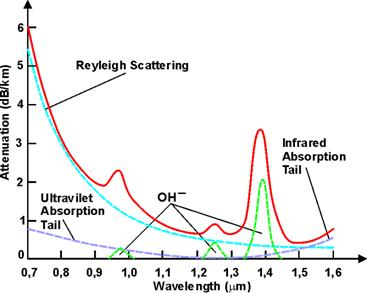
\includegraphics[scale=0.8]{figure/attenuation_curve.jpg}}
		\caption{Wavelength versus attenuation curve.}
		\label{fig:attenuation_curve}
	\end{figure}



\section{Artificial Neural Network(ANN)}
The study of the human brain is thousands of years old. With the advent of modern electronics, it was only natural to try to harness this thinking process. The first step toward artificial neural networks came in 1943 when Warren McCulloch, a neurophysiologist, and a young mathematician, Walter Pitts, wrote a paper on how neurons might work. They modeled a simple neural network with electrical circuits. Neural networks, with their remarkable ability to derive meaning from complicated or imprecise data, can be used to extract patterns and detect trends that are too complex to be noticed by either humans or other computer techniques. A trained neural network can be thought of as an "expert" in the category of information it has been given to analyses. Other advantages include:
\begin{itemize}
	\item Adaptive learning: An ability to learn how to do tasks based on the data given for training or initial experience.
	\item Self-Organization: An ANN can create its own organization or representation of the information it receives during learning time.
	\item Real Time Operation: ANN computations may be carried out in parallel, and special hardware devices are being designed and manufactured which take advantage of this capability.
	\item Fault Tolerance via Redundant Information Coding: Partial destruction of a network leads to the corresponding degradation of performance. However, some network capabilities may be retained even with major network damage.
\end{itemize}

\section{What is ANN}
Artificial Neural Network are computers whose architecture is modeled after the brain. They typically consist of hundreds of simple processing units which are wired together in a complex communication network. Each unit or node is a simplified model of real neuron which sends off a new signal or fires if it receives a sufficiently strong Input signal from the other nodes to which it is connected.Traditionally neural network was used to refer as network or circuit of biological neurons, but modern usage of the term often refers to ANN. ANN is mathematical model or computational model, an information processing paradigm i.e. inspired by the way biological nervous system, such as brain information system. ANN is made up of interconnecting artificial neurons which are programmed like to mimic the properties of m biological neurons. These neurons working in unison to solve specific problems. ANN is configured for solving artificial intelligence problems without creating a model of real biological system. ANN is used for speech recognition, image analysis, adaptive control etc. These applications are done through a learning process, like learning in biological system, which involves the adjustment between neurons through synaptic connection. Same happen in the ANN. Figure \ref{ANN} shows basic structure of Artificial Neural Network.
\begin{figure}[htbp]
	\centering{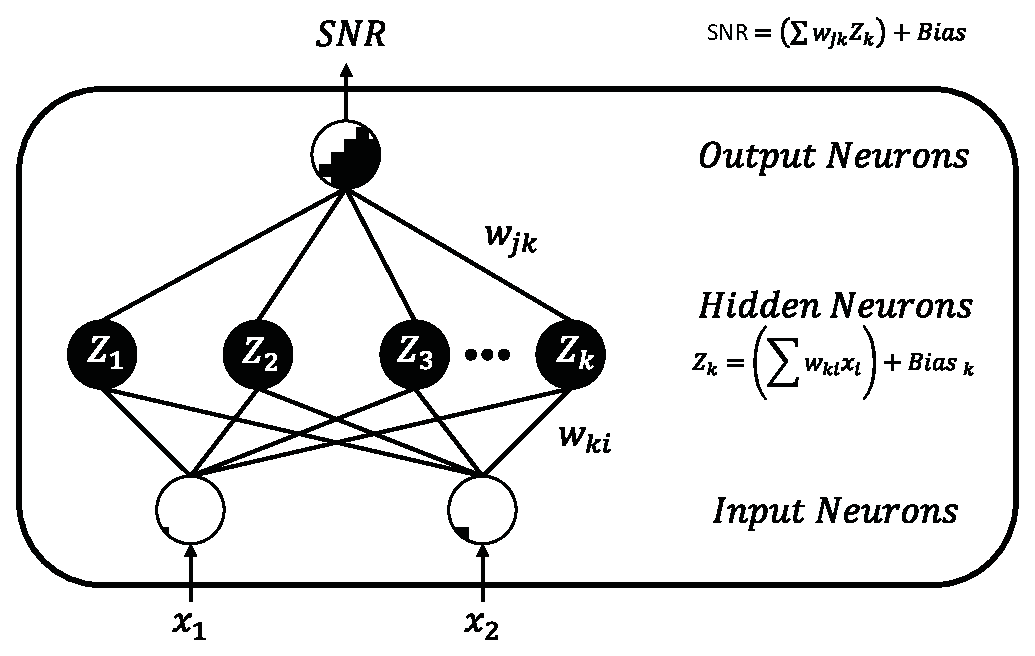
\includegraphics[scale=0.4]{figure/ANN.eps}}
	\caption{Example of Artificial Neural Network}
	\label{ANN}
\end{figure}
\section{Advantages of ANN}
There are various advantages of ANN over conventional approaches. Depending on the nature of the application and the strength of the internal data patterns can be generally expect a network to train quite well. This applies to problems where the relationships may be quite dynamic or non-linear. ANNs provide an analytical alternative to conventional techniques which are often limited by strict assumptions of normality, linearity, variable independence etc. Because an ANN can capture many kinds of relationships it allows the user to quickly and relatively easily model phenomena which may have been very difficult or impossible to explain otherwise.
\iffalse
\section{Conclusion}
Optical fiber communication is a complex system with lot of equipment. Analysis of them is much challenging. On the other hand ANN is a power full tool to model complex system. with the application of both great things can be done.
\fi
\chapter{PROPOSED OSNR MONITORING TECHNIQUE}
\section{Introduction}
The quality of the optical signal is generally assed by means of optical signal to noise ratio (OSNR) which is defined as the ratio of optical signal power to the ASE noise power in a reference bandwidth. OSNR is one of the key parameter which enables fault management of optical transmission system and networks. The OSNR limits is one of the key parameters that determine how far a wavelength can travel prior to regeneration. There are several methods of OSNR monitoring such as
\begin{itemize}
	\item Split-Symbol Moments Estimator (SSME)
	\item Maximum-likelihood (ML) Estimator for SNR.
	\item Squared signal to noise variance estimator (SNV).
	\item Second and fourth order moments estimator.
	\item Signal to variance ratio estimator.
\end{itemize}
Among them Second and fourth order moments method is of our interest. Advantages of second and fourth order moments methods are:
a) The performance of such OSNR estimation is inherently insensitive to the phase noise of transmitter LASERs and local oscillators, since it involves only the measurement of second and fourth order moments only.
b) It is not affected by linear fiber transmission impairments such as chromatic dispersion (CD) and polarization mode dispersion (PMD), because OSNR estimation is done after adaptive equalization.
\section{Conventional Second and Fourth Order Moments Method}
Coherent optical receiver employing phase and polarization diversities and typical DSP stages for data recovery in polarization-division multiplexed transmission systems .For OSNR monitoring, we use the signal at the adaptive equalizer output. The digital filters used in the equalizer can compensate for a large amount of linear fiber transmission impairments without any notable penalty and the signal at this stage is mainly contaminated by ASE noise. Therefore, the output of the adaptive equalizer is the earliest stage of the DSP chain where the OSNR estimation is done. In addition, DSP stages for frequency-offset compensation and carrier-phase estimation can be placed after the OSNR estimation stage. The output signal from the adaptive filter can be approximated as
\begin{align}
Yn \approx \sqrt{C}a_n e^{j\theta_n}+\sqrt{N}W_n
\end{align}
Where $a_n$ is the M-PSK or M-QAM symbol amplitude, C the signal-power scale factor, N the noise-power scale factor, $W_n$ the ASE noise, $\theta_n$ the phase noise stemming from phase fluctuation of a transmitter laser and a local oscillator, and n the number of samples,

The second order moment $M_2$ of $Y_n$ can be expressed as
\begin{equation}\label{eq:2}
\begin{aligned}
M_2 &=E\{y_n y_n^*\}\\
&=CE\{a_n e^{j\theta_n} a_n^* e^{-j\theta_n}\}+\sqrt{CN}E\{a_n e^{j\theta_n} W_n\}+NE\{w_n w_n^*\}\\
&=CE\{|a_n|^2\}+\sqrt{CN}(E\{a_n e^{j\theta_n} W_n^*\}+E\{a_n^* e^{-j\theta_n} W_n\})+NE\{w_n w_n^*\}
\end{aligned}
\end{equation}
Where E \{-\} represents the ensemble average and the superscript (-)* denotes the complex conjugate. Since the signal and the noise obey a mutually-independent complex-valued stochastic process, we have
\begin{align}
E\{a_n e^{j\theta_n} W_n^*\}=0\\
E\{a_n^* e^{-j\theta_n} W_n\}=0
\end{align}
We also assume that the signal $a_n$ and the noise $W_n$ are normalized to have an equal variance given by, 
\begin{align}
\{E\{|a_n|^2\}\}=\{E\{|W_n|^2\}\}=v
\end{align}
Thus, we can rewrite Eq.\ref{eq:2} as
\begin{align}
\label{eq:6}
M_2 = v(C+N)
\end{align}
And the signal to noise ratio (CNR) is expressed as
\begin{align}\label{eq:7}
SNR=\frac{C}{N}
\end{align}
On the other hand, the fourth-order moment $M_4$ of $y_n$ can be written as
\begin{equation}\label{eq:8}
\begin{aligned}
M_4&=E\{(y_n y_n^*)^2\}\\
&=C^2E\{(a_n a_n^*)^2\}+2C\sqrt{CN}(E+E\{a_n a_n^* a_n^* e^{-j\theta_n}W_n\})+CN(E\{(a_n e^{j\theta_n W_n^*})^2\}\\&+4E\{a_n a_n^* W_n W_n^*\}+E\{(a_n^* e^{-j\theta_n}W_n)^2\})+2C\sqrt{CN}(E\{W_n W_n^* a_n e^{j\theta_n}W_n^*\}\\&+E\{W_n W_n^* a_n e^{-j\theta_n }W_n^*\})+N^2E\{(W_n W_n^*)^2\}
\end{aligned}
\end{equation}
In Eq.\ref{eq:8}, since
\begin{align}
E\{a_n\}=E\{a_n^*\}=E\{W_n\}=E\{W_n^*\}=0\\
E\{a_n a_n^* a_n e^{j\theta_n} W_n^*\}=0\\
E\{W_n W_n^* a_n e^{j\theta_n} W_n^*\}=0\\
E\{a_n a_n^* a_n^* e^{-j\theta_n} W_n\}=0\\
E\{W_n W_n^* a_n^* e^{-j\theta_n} W_n\}=0
\end{align}
Also note that the real part $a_{nl}$ and the imaginary part $a_{nQ}$ of $a_n$ are uncorrelated in M-ary PSK and M-ary QAM signals when $M\geq 4$. Then we find that
\begin{align}
E\{(a_n e^{j\theta_n}W_n^*)^2\}=E\{a_n^2\}. E\{(e^{j\theta_n} W_n^*)^2\}=0
\end{align}
Because
\begin{align}
E\{a_n^2\}=E\{a_{nl}^2-a_{nQ}^2+2ja_{nl} a_{nQ}\}=0
\end{align}
Similarly, we have
\begin{align}
E\{(a_n e^{-j\theta_n}W_n^*)^2\}=E\{(W_n e^{-j\theta_n})^2\}.E\{(a_n^*)^2\}=0
\end{align}
In addition it is evident that
\begin{align}
E\{(a_n a_n^*)^2\}=E\{|a_n|^4\}\\
E\{(w_n w_n^*)^2\}=E\{|w_n|^4\}\\
E\{a_n a_n^* w_n w_n^*\}=E\{|a_n|^2 |w_n|^2\}
\end{align}
Taking all of these equations into consideration, we can simplify Eq.\ref{eq:8} as
\begin{equation}\label{eq:20}
	\begin{aligned}
		M_4&=C^2E\{|a_n|^4\}+4CNE\{|a_n|^2 |w_n|^2\}+N^2E\{|w_n|^4\}\\
		&=k_a v^2 C^2 +4v^2CN+k_w v^2N^2
	\end{aligned}
\end{equation}
Where
\begin{align}
	k_a=\frac{E\{|a_n|^4\}}{E\{|a_n|^2\}^2}\\
	k_w=\frac{E\{|w_n|^4\}}{E\{|w_n|^2\}^2}
\end{align}
Are kurtoses of the signal and the noise respectively, The Gaussian distribution of ASE noise yields $k_w=2$.

Solving Equations \ref{eq:6} and \ref{eq:20}, we obtain
\begin{align}\label{eq:23}
	C=\frac{1}{v} \sqrt{\frac{2M_2^2 -M_4}{2-k_a}}
	\end{align}
\begin{align}\label{eq:24}
	N=\frac{1}{v}\{M_2- \sqrt{\frac{2M_2^2 -M_4}{2-k_a}}\}
\end{align}
Therefore, determining $M_2$ and $M_4$ from exponential results and using Eqs. \ref{eq:7}, \ref{eq:23} and \ref{eq:24}, we can estimate CNR as
\begin{align}\label{eq:snr}
	SNR=\frac{\sqrt{2M_2^2 -M_4}}{M_2\sqrt{2-k_a}-\sqrt{2M_2^2 -M_4}}
\end{align}
In a practical system, we can calculate second and fourth order moments from a received data block of L symbols as
\begin{align}\label{eq:m2}
M_2\approx\frac{1}{L}\sum_{n=0}^{L-1}|y_n|^2
\end{align}
\begin{align}\label{eq:m4}
M_4\approx\frac{1}{L}\sum_{n=0}^{L-1}|y_n|^4
\end{align}

Respectively, As shown in Eqs. \ref{eq:m2} and \ref{eq:m4}, measuring second- and fourth order moments does not include any effect of the phase noise and thus the proposed scheme operates phase insensitively.

Equation \ref{eq:snr} is a generalized equation to calculate SNR of any arbitrary modulation format. The value of $k_a$ is dependent on the modulation format; for example, in the case of QPSK, we have $k_a=1$ since,$a_n\in\{1,-1,j,-j\}$

Then SNR is expressed as
\begin{align}
	SNR_{QPSK}=\frac{\sqrt{2M_2^2 -M_4}}{M_2-\sqrt{2M_2^2 -M_4}}
\end{align}
On the other hand, for the 16-QAM signal, since $a_n\in\{\pm 1 \pm i, \pm 1 \pm 3i, \pm 3 \pm i, \pm 3 \pm 3i\}, k_a=1.32$

Then, SNR is given as
\begin{align}\label{eq:snr16qam}
SNR=\frac{\sqrt{2M_2^2 -M_4}}{M_2\sqrt{0.68}-\sqrt{2M_2^2 -M_4}}
\end{align}

\section{Relationship Between SNR and OSNR}
To estimate the OSNR from SNR the following relation is ideally considered []:

\begin{align}\label{eq:snrvsosnr}
OSNR=\frac{p R_s}{2 B_{ref}}SNR
\end{align}

where, Rs is the symbol rate and $R_s/B_ref$ is an adjustment factor to measure noise bandwidth to the reference bandwidth Bref. The reference bandwidth $B_ref$ is usually set to 12.5 GHz, which is equivalent to the 0.1-nm OSA resolution bandwidth. The value of p is 1 for single-polarized signal whereas 2 for polarization-multiplexed signal.

In Eq. \ref{eq:snrvsosnr}, only the ASE noise is considered. However, there are other sources of noise from transceiver. In such case, the relationship can be expressed as follow []:

\begin{align}\label{eq:snrvsosnr2}
\frac{1}{SNR}=\zeta \frac{1}{OSNR}+\eta
\end{align}

where, $\zeta$ is a proportionality constant between SNR and OSNR and $\eta$ is attributed from background noise of transceiver. The value of $\zeta$ and $\eta$ can be estimated accurately by curve fitting method with a known SNR and OSNR measurement set. Therefore, estimation of OSNR is only depend on proper estimation of SNR and in the rest of this paper, results for SNR estimation are depicted.

\section{Problems of Conventional Method}
Conventional second and fourth order moments method can estimate OSNR with low error for 4-QAM signal for all value of SNR. This shown in Figure \ref{fig:4-qam-error}.
\begin{figure}[htbp]
	\centering{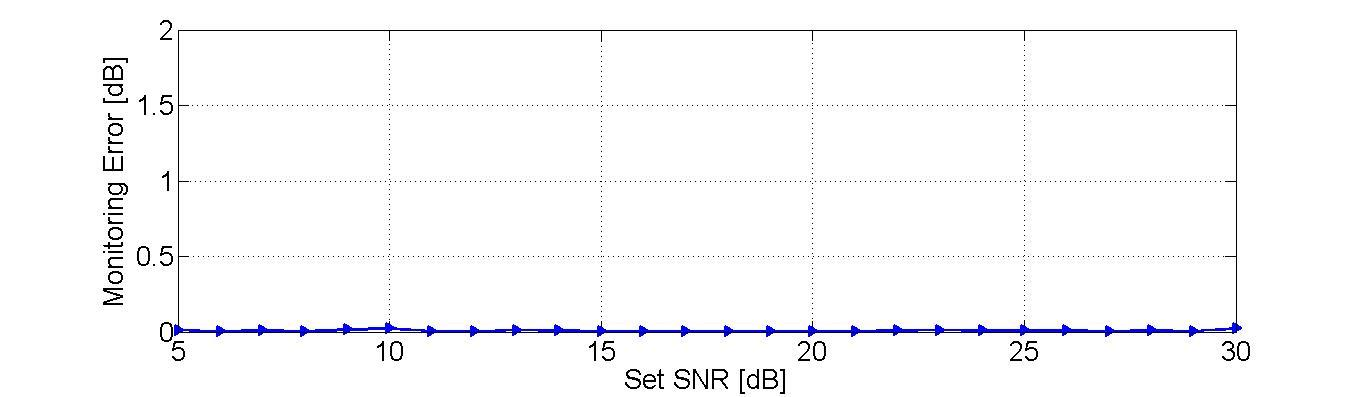
\includegraphics[scale=0.9]{figure/four-qam-error.jpg}}
	\caption{Set SNR versus Monitoring Error curve for 4-QAM}
	\label{fig:4-qam-error}
\end{figure}

Estimation of SNR by $M_2 M_4$ method for high SNR provides large error for higher order QAM, if the SNR increases to a higher value. A graph of varying SNR and estimated error is shown in Figure \ref{fig:standardm2m4error}.
\begin{figure}[htbp]
	\centering{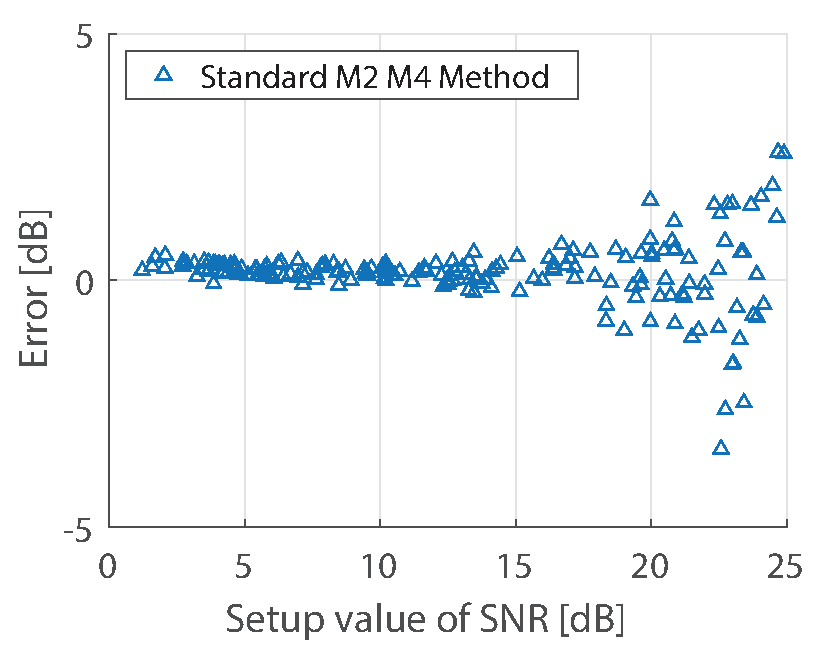
\includegraphics[scale=0.7]{figure/16qamstandardM2M4error.eps}}
	\caption{Set SNR versus Error curve of 16-QAM by conventional second and fourth order moment method.}
	\label{fig:standardm2m4error}
\end{figure}

It is clear from Figure \ref{fig:standardm2m4error} that conventional second and fourth order method of estimation of SNR can estimate low SNR easily. For high SNR the corresponding error is high. In this literature our main aim is to develop a method such that higher SNR can estimated correctly at the receiver end keeping the advantages of conventional $M_2 M_4$ method.

\section{Principle of Proposed Technique}
From the above discussion it is evident that second and fourth order moments method is not suitable for high SNR estimation, but it is good for 4-QAM. A modification in the SNR monitoring technique and using the formula of 4-QAM of current second and fourth order method this problem can be solved.
\begin{figure}[htbp]
	\centering{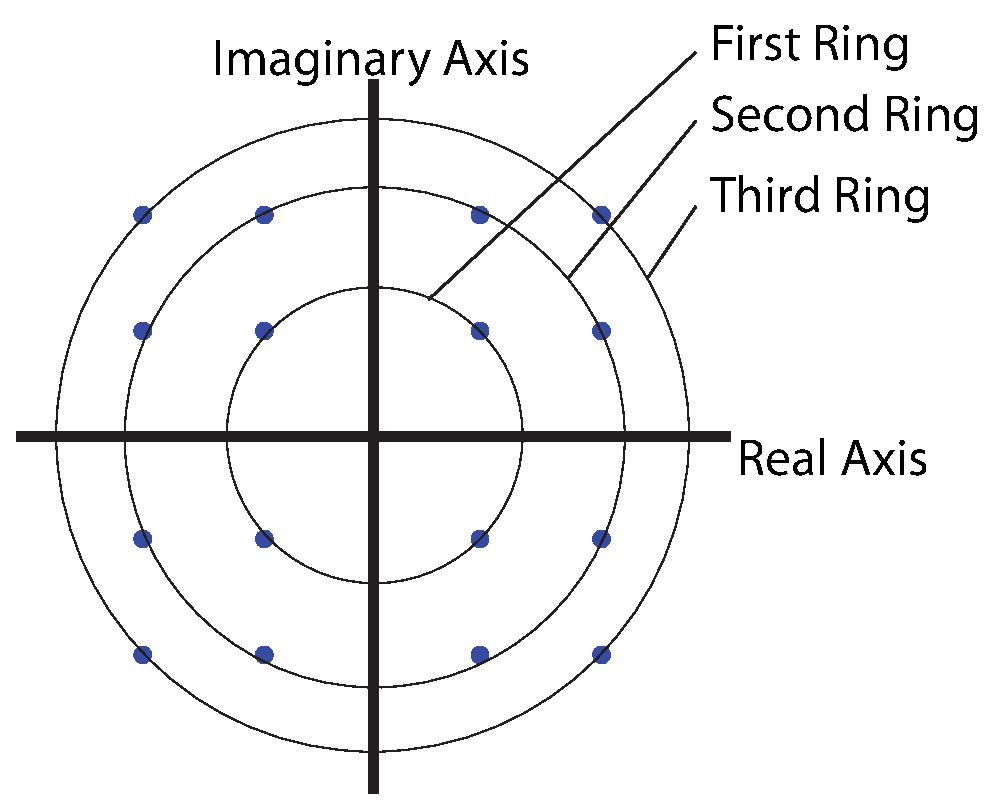
\includegraphics[scale=0.45]{figure/qam16_constallation.eps}}
	\caption{Constellation diagram of 16-QAM.}
	\label{fig:qam16-constallation}
\end{figure}
Constellation diagram of 16-QAM is shown in Figure \ref{fig:qam16-constallation} It is seen that there are three circle in the constellation diagram. There are three class of ring according to the symbol power of 16-QAM modulation format.  By taking mid point of two consecutive circle both side of middle circle as threshold and comparing the incoming data we can easily extract the data of  middle circle. If we calculate variance, which is defined as:
\begin{align}\label{eq:variance}
V_m = \frac{1}{L}\sum_{n=1}^{L}(|y_m (n)|-\sqrt{P_m})^2
\end{align}
where ym(n) are the middle-ring constellation points which are separated using appropriate thresholding method from all symbols [10] and Pm is the average power of middle ring
symbols.

 The variations of $V_m$ for different SNR values for 16-QAM is shown in Figure \ref{fig:mmsVsSNR}. Clear variation in the value with change in SNR is visible. This can help to estimate SNR. But this data is not consistent in the lower SNR.
\begin{figure}[htbp]
	\centering{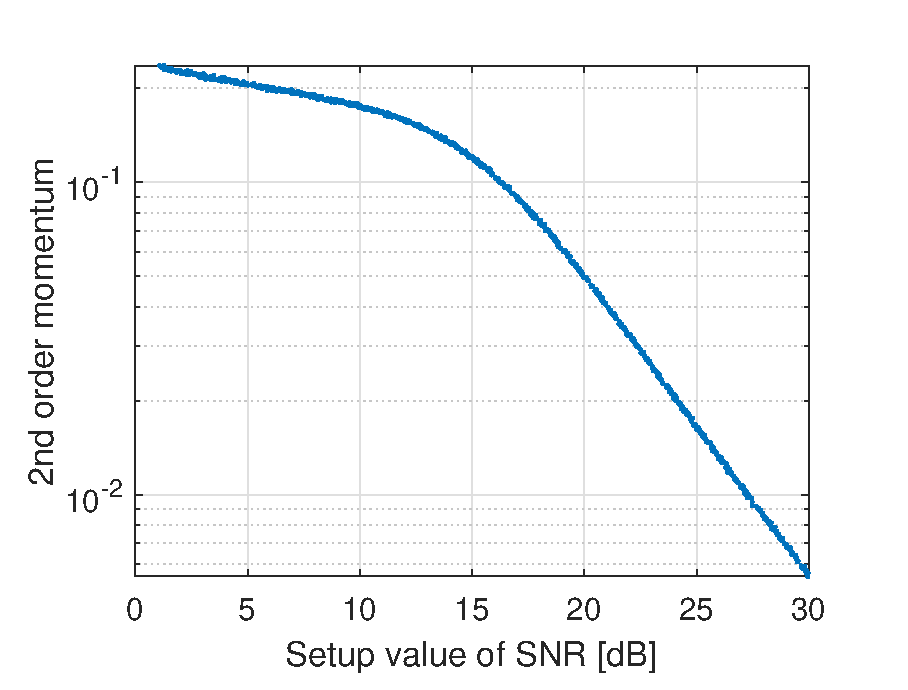
\includegraphics[scale=0.7]{figure/mmsVsSNR.eps}}
	\caption{Set SNR versus variance of magnitude curve of extracted data from middle circle of 16-QAM.}
	\label{fig:mmsVsSNR}
\end{figure}
On the other hand 2nd order momentum($M_2$) of all data versus SNR plot shows clear variation for lower SNR but not for higher SNR as shown in Figure \ref{fig:m2sVsSNR}.  
\begin{figure}[htbp]
	\centering{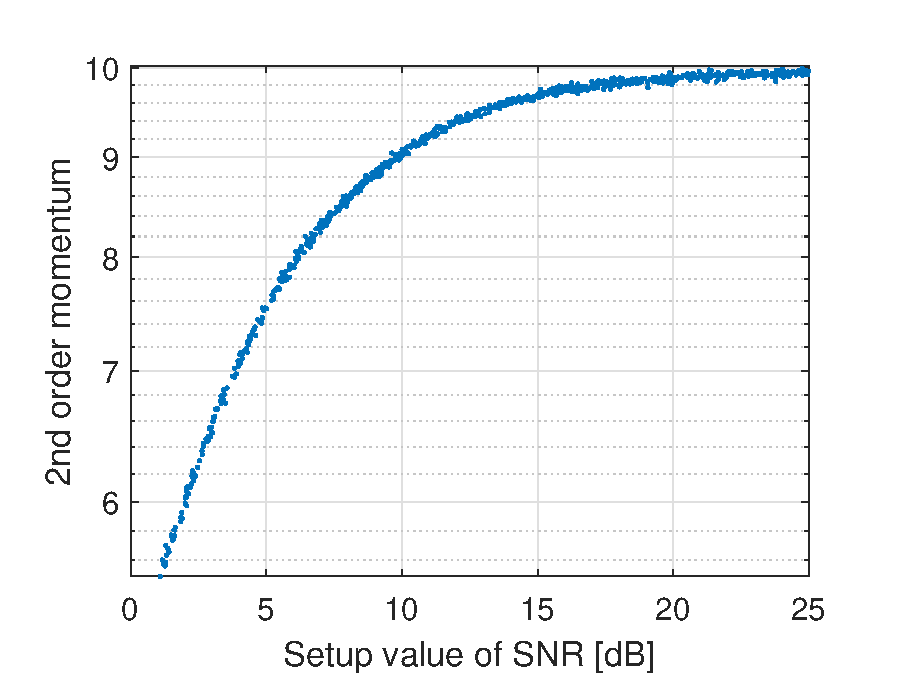
\includegraphics[scale=0.7]{figure/m2sVsSNR.eps}}
	\caption{Set SNR versus 2nd order momentum curve of all data of 16-QAM.}
	\label{fig:m2sVsSNR}
\end{figure}
Combination of both information can give us better estimation of SNR. But driving equation using this results is not easy specially for higher order modulation. So our aim is to train a neural network with this data to estimate the SNR.
\iffalse
\section{Conclusion}
\fi
\chapter{SIMULATION RESULTS AND DISCUSSION}
\iffalse
\section{Introduction}
In order to confirm the effectiveness of our proposed method for estimating SNR, we conduct computer simulations under some conditions explained latter. Data has been generated to train the Neural Network model.
\fi
\section{Simulation setup}
\begin{figure}[htbp]
	\centering{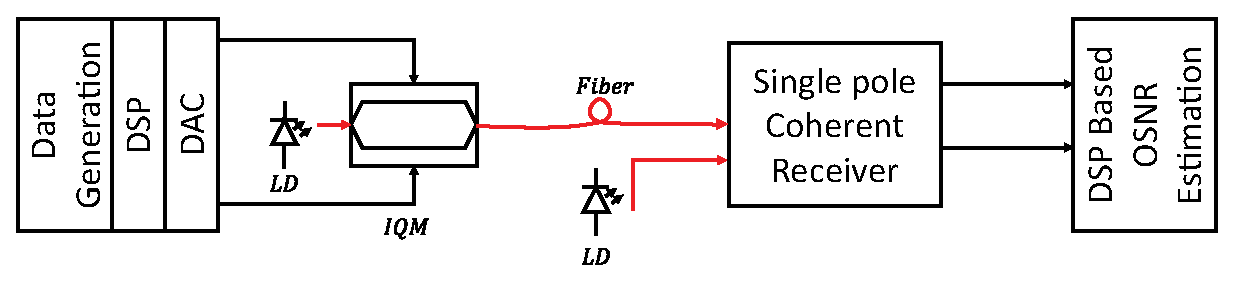
\includegraphics[scale=0.7]{figure/block.eps}}
	\caption{Schematic of simulation setup to verify the proposed method.}
	\label{fig:simulation_setup}
\end{figure}
\iffalse
In the simulation, each wavelength channel consists of a dual polarization single-carrier 25-Gbaud QPSK signal or a dual-polarization single-carrier 25-Gbaud 16-QAM signal .At the transmitter , the spectrum of the signal on each carrier or subcarrier is shaped by the Nyquist filter with a roll of factor of 0.5.The channel thus obtained are aligned in the frequency domain without any guard band. As system impairments, CD, the laser phase noise, and the ASE noise take into account. Assuming that the ASE noise as white Gaussian noise, we control SNR by changing its average power. At the receiver side, the signal is received by an optical homodyne receiver and delivered to the DSP circuit. In the DSP circuit, the signal on each carrier or subcarrier are separated by the Nyquist filter with a roll of factor of 0.5; then, the separated signal is eight fold over sampled and fed into a 21-tap half symbol spaced finite impulse response filter, which is adapted by the constant modulus algorithm (CMA) for the QPSK signal or the radial directed equalization (RDE) algorithm for the 16-QAM signal.
\fi
For the simulation, first random 16-QAM/64-QAM signal is generated and root-raised cosine (RRC) filtering is used to reshape the pulse. The signal is then modulated using IQ modulator with a distributed feedback laser (DFB) of 1MHz linewidth and central wavelength of 1550 nm.The modulated signal is then passed through a 50-km standard single mode fiber (SMF) which has an attenuation coefficient of 0.2dB/km and chromatic dispersion coefficient of 17 ps/nm-km. additive white Gaussian noise (AWGN) is added, before received the signal using a single-polarization phase diversity coherent receiver.
\section{Preparing Data}
The simulation was run for randomly selected SNR ranging from 1dB to 30dB. All data from each iteration then saved in a database as shown in Table \ref{table:dataset}. 1000 data sample was prepared. 800 data sample was is used for training and 200 data was used for only testing purpose.
\begin{table}[h!]
	\caption{Data prepared for training.}
	\begin{center}
		\centering
		\begin{tabular}{ |p{3cm}|p{3cm}|p{3cm}|p{3cm}| } 
			\hline
			\hfil Iteration & \hfil $M_2$ & \hfil Variance & \hfil SNR \\ 
			\hline
			\hfil 1 & \hfil 9.01 & \hfil 0.17 & \hfil 9.98 \\ 
			\hline
			\hfil 2 & \hfil 8.76 & \hfil 0.18 & \hfil 8.63 \\ 
			\hline
			\hfil 3 & \hfil 9.78 & \hfil 0.10 & \hfil 16.03 \\ 
			\hline
			\hfil 4 & \hfil 9.84 & \hfil 0.05 & \hfil 19.63 \\ 
			\hline
			\hfil .. & \hfil .. & \hfil .. & \hfil .. \\ 
			\hline
			\hfil .. & \hfil .. & \hfil .. & \hfil .. \\ 
			\hline
			\hfil 1000 & \hfil 9.83 & \hfil 0.08 & \hfil 17.64 \\ 
			\hline
		\end{tabular}
		\label{table:dataset}
	\end{center}
\end{table}
\section{Training Model}
\begin{figure}[htbp]
	\centering{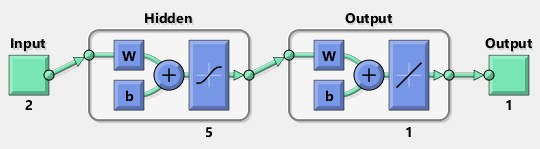
\includegraphics[scale=0.8]{figure/net.jpg}}
	\caption{Structure of Neural Network used in the simulation.}
	\label{fig:net}
\end{figure}
Figure \ref{fig:net} shows the structure of the ANN used in the simulation. Using matlab "\textit{feedforwardnet}" the Network was trained with the data. Here is the details structure of the neural network:

Neural Network\\
name: 'Feed-Forward Neural Network'\\
userdata: Train data\\

Dimensions:\\
numInputs: 1\\
numLayers: 2\\
numOutputs: 1\\
numInputDelays: 0\\
numLayerDelays: 0\\
numFeedbackDelays: 0\\
numWeightElements: 21\\
sampleTime: 1\\

Connections:\\{\tiny }
biasConnect: [1; 1]\\
inputConnect: [1; 0]\\
layerConnect: [0 0; 1 0]\\
outputConnect: [0 1]\\

Subobjects:\\
input: Equivalent to inputs{1}\\
output: Equivalent to outputs{2}\\
inputs: {1x1 cell array of 1 input}\\
layers: {2x1 cell array of 2 layers}\\
outputs: {1x2 cell array of 1 output}\\
biases: {2x1 cell array of 2 biases}\\
inputWeights: {2x1 cell array of 1 weight}\\
layerWeights: {2x2 cell array of 1 weight}\\

Functions:\\
adaptFcn: 'adaptwb'\\
adaptParam: (none)\\
derivFcn: 'defaultderiv'\\
divideFcn: 'dividerand'\\
divideParam: .trainRatio, .valRatio, .testRatio\\
divideMode: 'sample'\\
initFcn: 'initlay'\\
performFcn: 'mse'\\
performParam: .regularization, .normalization\\
plotFcns: {'plotperform', plottrainstate, ploterrhist, plotregression}\\
plotParams: {1x4 cell array of 4 params}\\
trainFcn: 'trainlm'\\
trainParam: .showWindow, .showCommandLine, .show, .epochs, .time, .goal, .min\_grad, .max\_fail, .mu, .mu\_dec, .mu\_inc, .mu\_max\\

Weight and Bias values:\\
IW: {2x1 cell} containing 1 input weight matrix\\
LW: {2x2 cell} containing 1 layer weight matrix\\
b: {2x1 cell} containing 2 bias vectors\\

Methods:\\
adapt: Learn while in continuous use\\
configure: Configure inputs \& outputs\\
gensim: Generate Simulink model\\
init: Initialize weights \& biases\\
perform: Calculate performance\\
sim: Evaluate network outputs given inputs\\
train: Train network with examples\\
view: View diagram\\
unconfigure: Unconfigure inputs \& outputs\\



\section{Results}
The results shows estimation using proposed method is more accurate then conventional $M_2M_4$ method for all SNR. 
\subsection{Results for 16-QAM}
Set SNR versus estimation error for 16-QAM is shown in Figure \ref{fig:snrVserror_proposed_16} and regression between set SNR and estimated SNR for 16-QAM is shown in Figure \ref{fig:regression_proposed_16}. Details results are discussed below: 
\begin{figure}[htbp]
	\centering{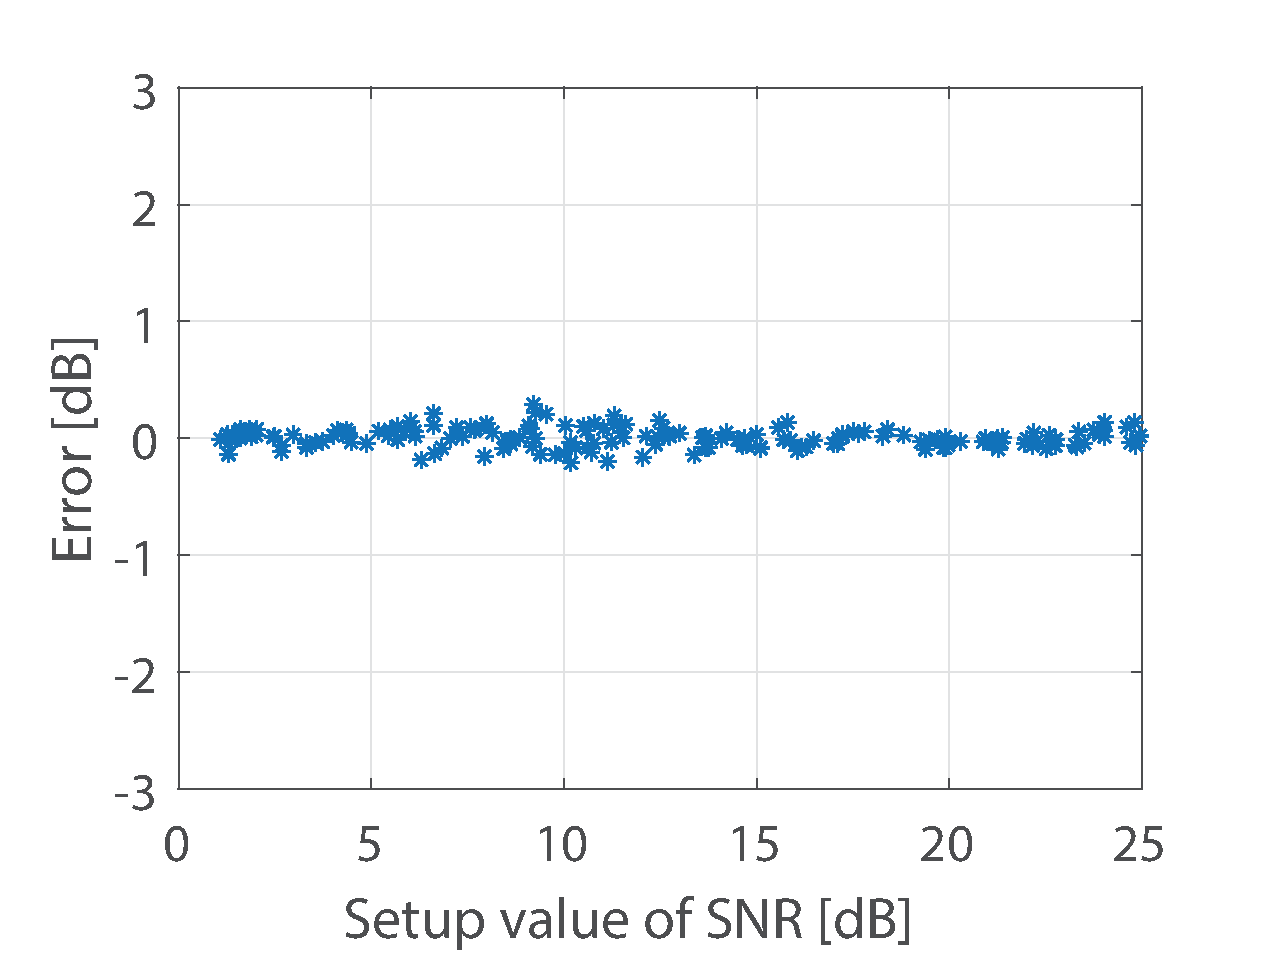
\includegraphics[scale=0.5]{figure/snrVserror_proposed_16.eps}}
	\caption{Set SNR versus estimation error result using proposed method for 16-QAM.}
	\label{fig:snrVserror_proposed_16}
\end{figure}
\begin{figure}[htbp]
	\centering{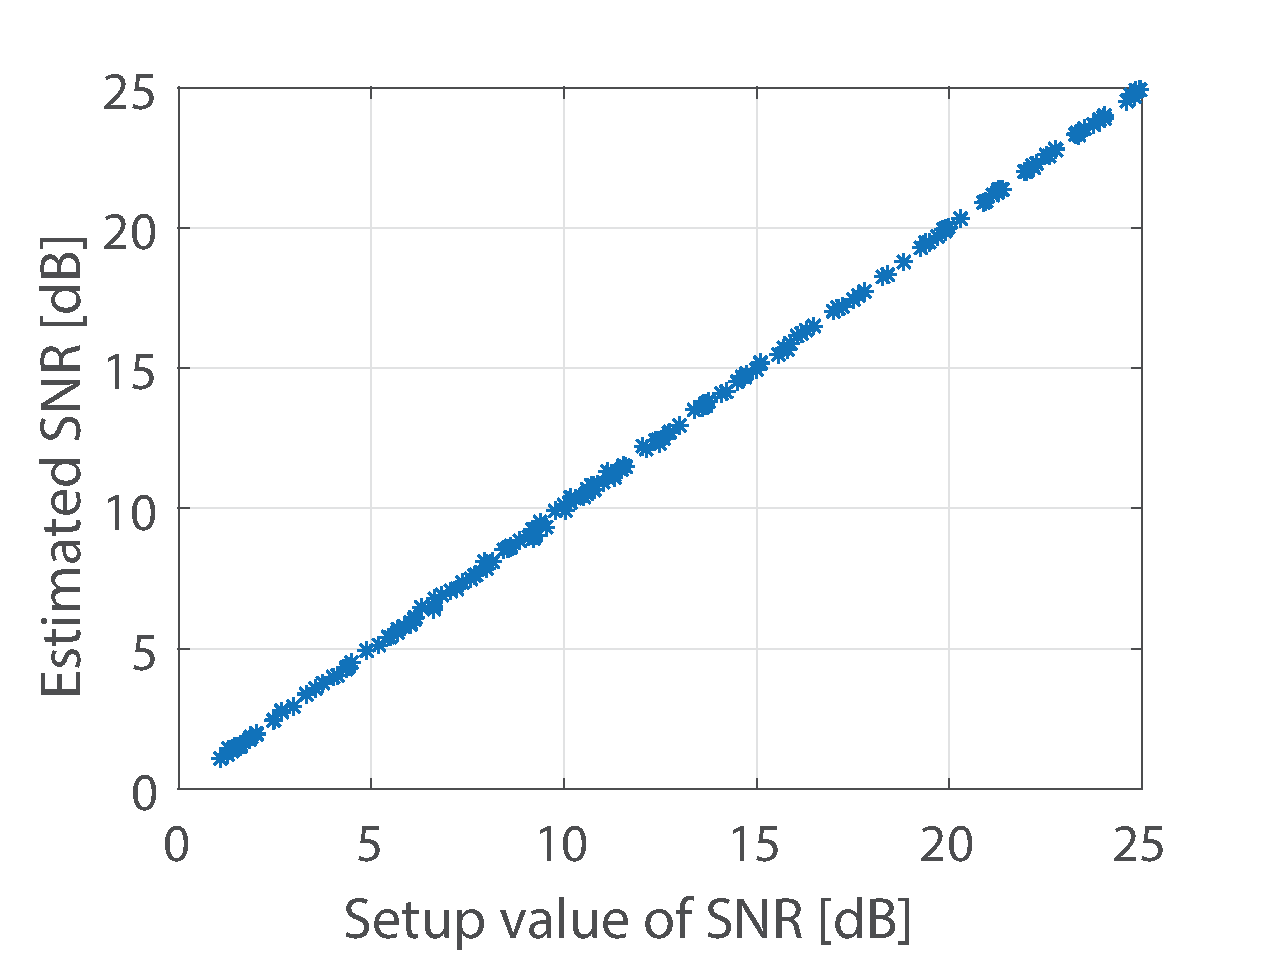
\includegraphics[scale=0.5]{figure/regration_proposed_16.eps}}
	\caption{Regression curve of proposed method for 16-QAM. }
	\label{fig:regression_proposed_16}
\end{figure}

Figure \ref{fig:error_compare_16qam} shows Comparison between conventional method and proposed method. In this figure it is clear that conventional $M_2M_4$ method is not accurate for higher SNR but proposed method is more accurate for SNR estimation for all SNR. Comparison of regression curve for 16-QAM between two methods is also shown in Figure \ref{fig:regression_compare_16qam}.
\begin{figure}[htbp]
	\centering{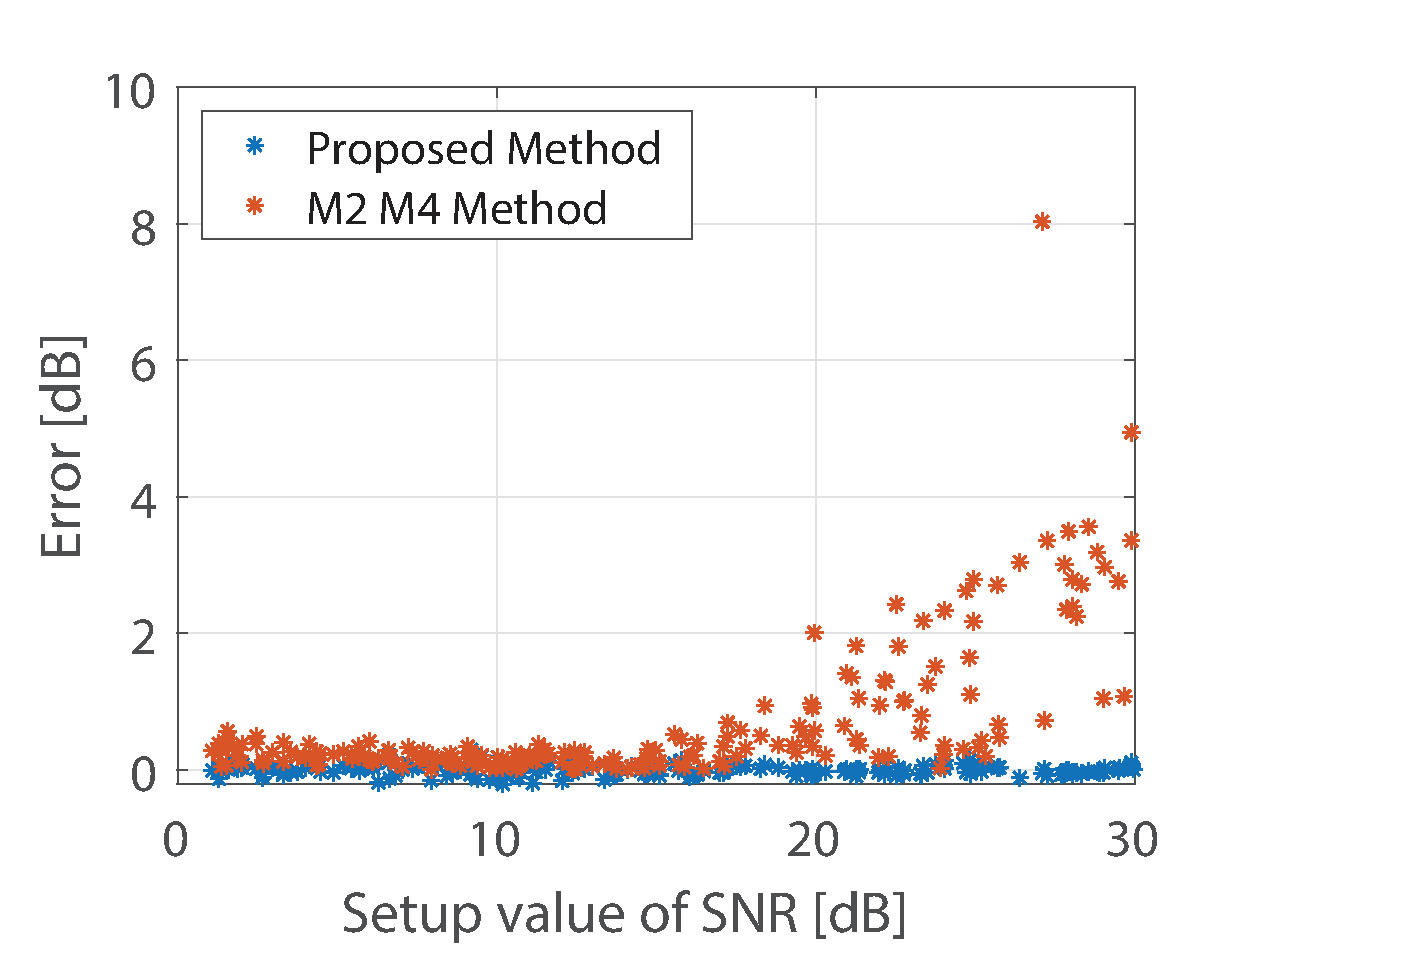
\includegraphics[scale=0.5]{figure/error_compare_16qam.eps}}
	\caption{Error Comparison of proposed method and $M_2 M_4$ method for 16-QAM. }
	\label{fig:error_compare_16qam}
\end{figure}
\begin{figure}[htbp]
	\centering{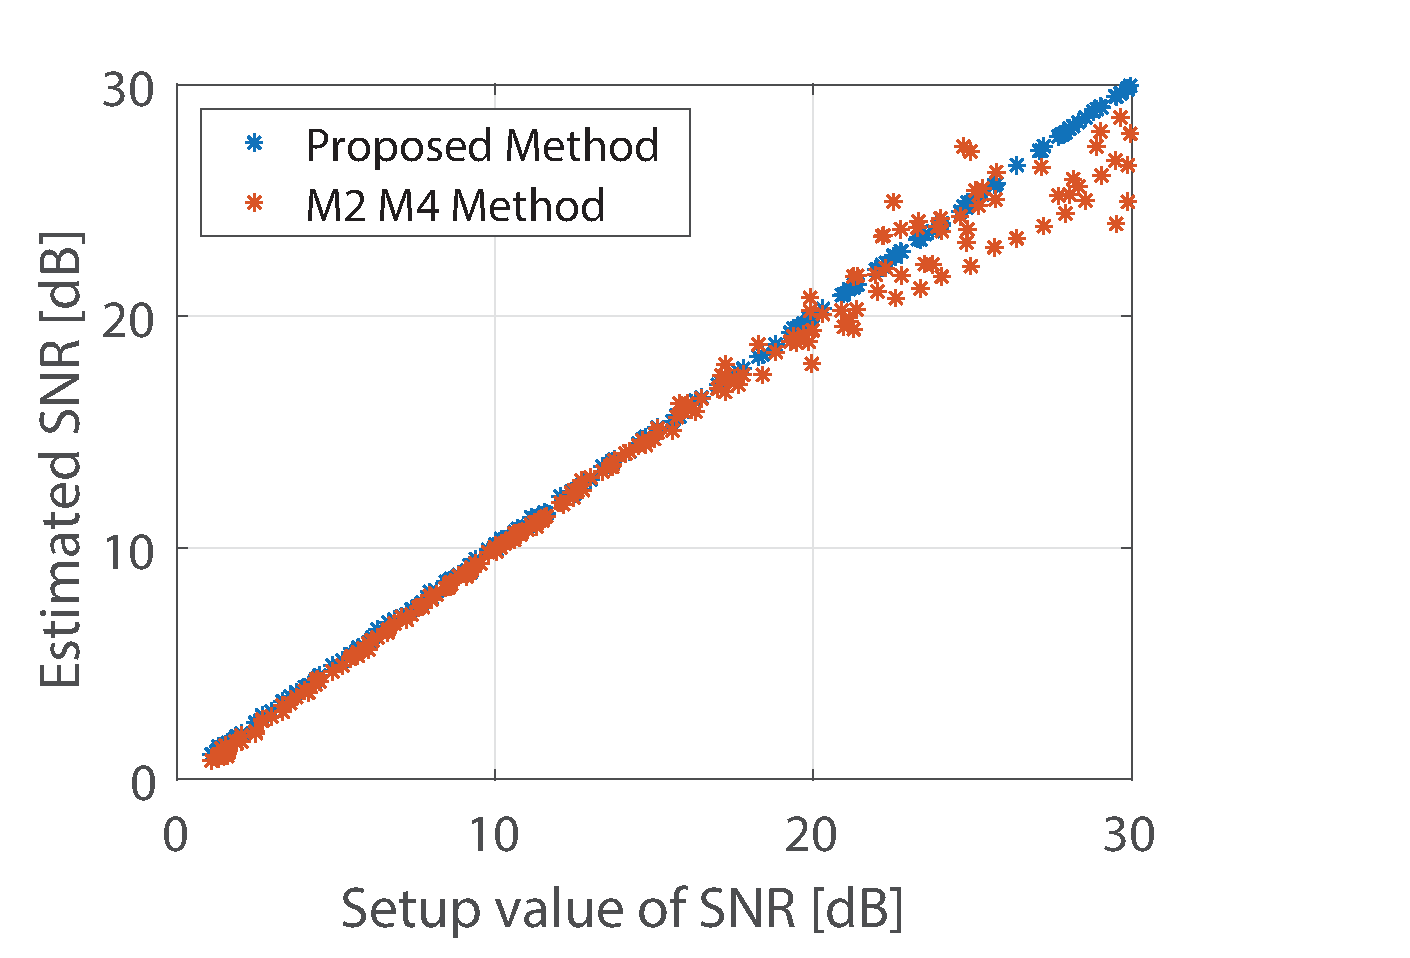
\includegraphics[scale=0.5]{figure/regression_compare_16qam.eps}}
	\caption{Regression Comparison of proposed method and $M_2 M_4$ method for 16-QAM. }
	\label{fig:regression_compare_16qam}
\end{figure}
\subsection{Results for 64-QAM}
Set SNR versus estimation error for 64-QAM is shown in Figure \ref{fig:error_proposed_64qam} and regression between set SNR and estimated SNR for 64-QAM is shown in Figure \ref{fig:regression_proposed_64qam}. 

\begin{figure}[htbp]
	\centering{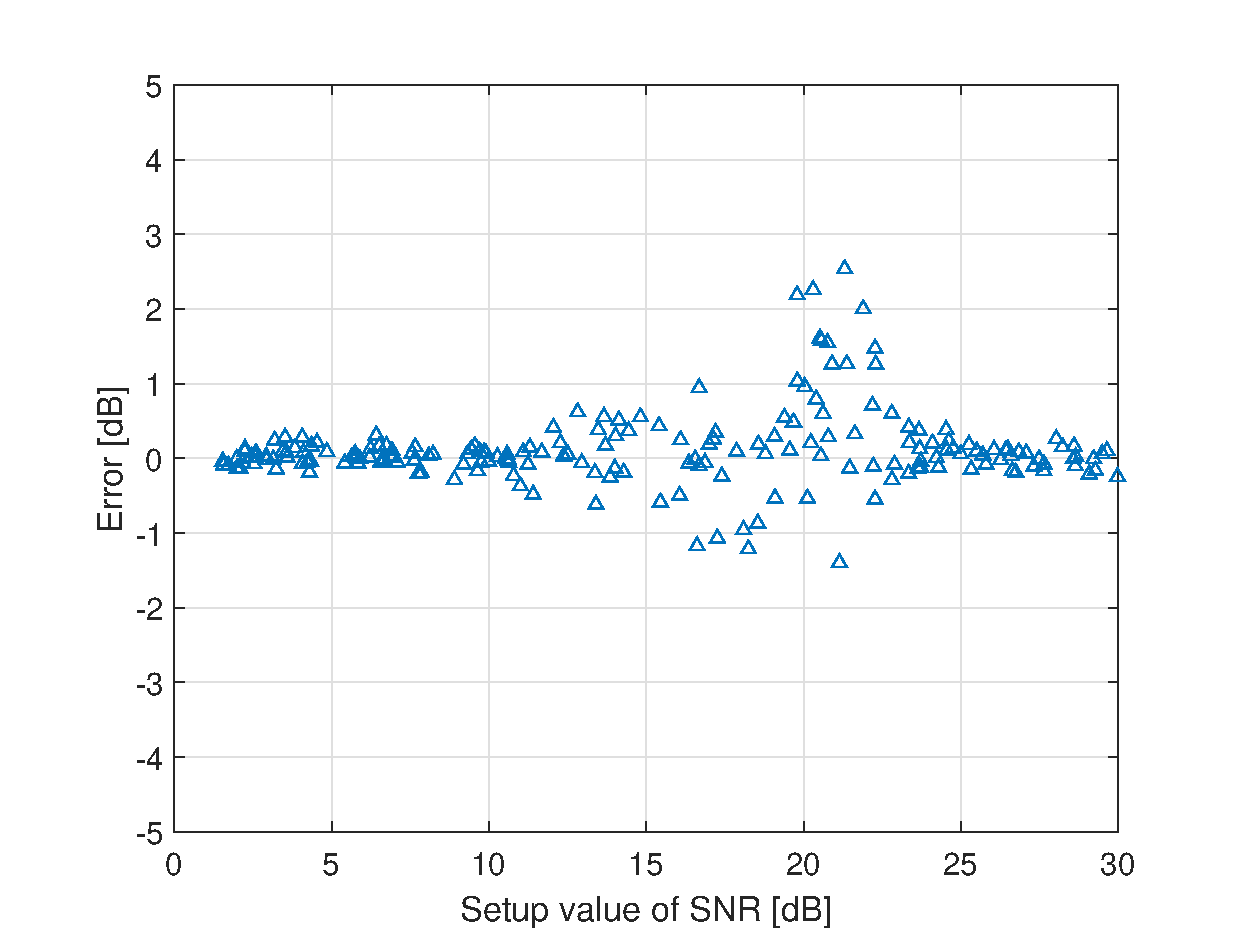
\includegraphics[scale=0.5]{figure/64_proposed_error.eps}}
	\caption{Set SNR versus estimation error result using proposed method for 64-QAM. }
	\label{fig:error_proposed_64qam}
\end{figure}
\begin{figure}[htbp]
	\centering{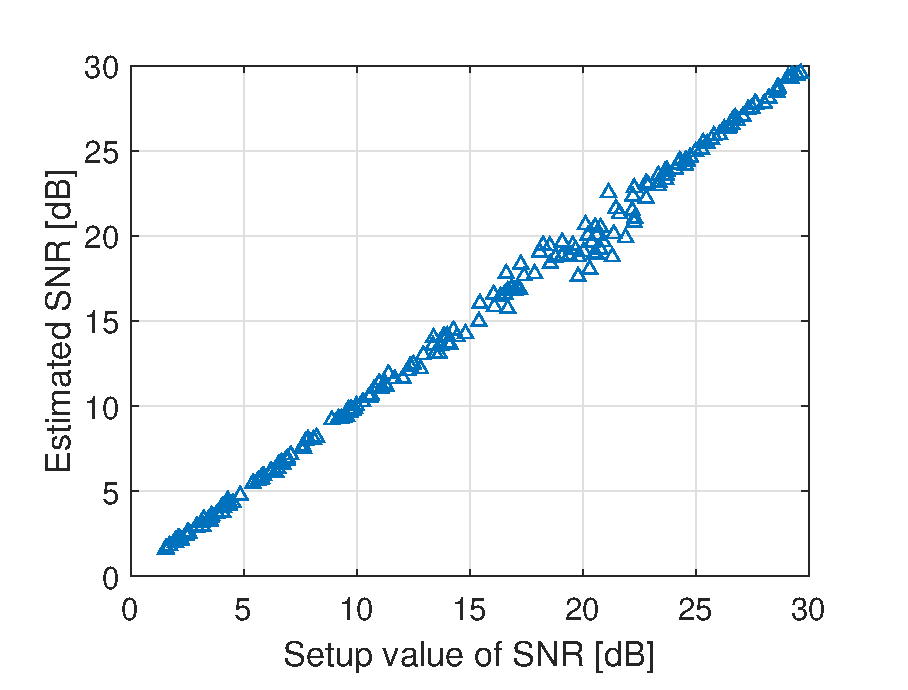
\includegraphics[scale=0.6]{figure/64_proposed_regression.eps}}
	\caption{Regression curve of proposed method for 16-QAM. }
	\label{fig:regression_proposed_64qam}
\end{figure}

Figure \ref{fig:error_compare_64qam} shows Comparison between conventional method and proposed method. In this figure it is clear that accuracy of conventional $M_2M_4$ method is less for higher SNR but accuracy of proposed method is higher for SNR estimation of all SNR. 
\begin{figure}[htbp]
	\centering{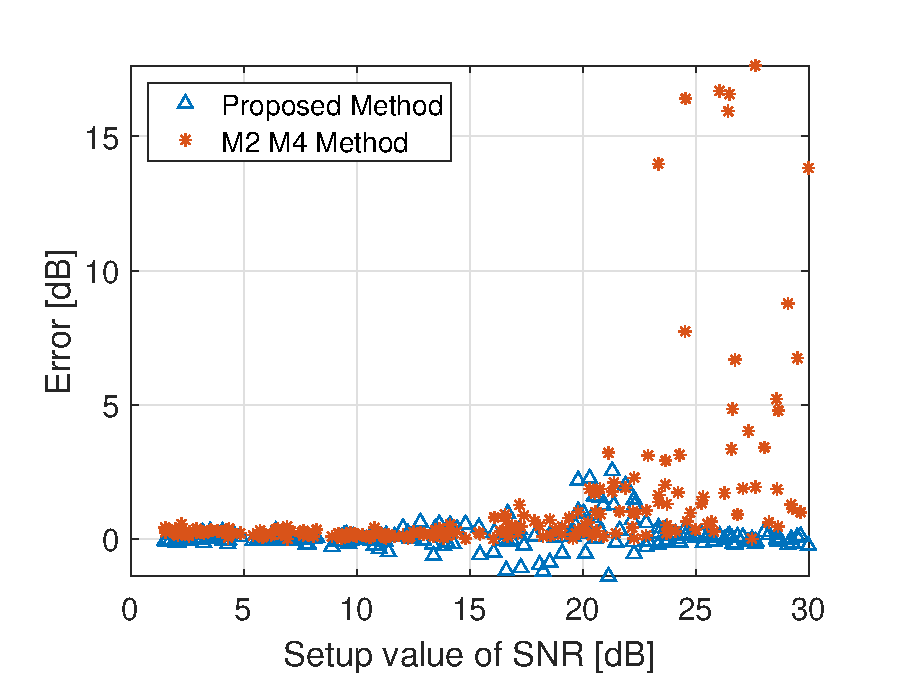
\includegraphics[scale=0.6]{figure/64_snrVsErrorCompare.eps}}
	\caption{Error Comparison of proposed method and $M_2 M_4$ method for 64-QAM. }
	\label{fig:error_compare_64qam}
\end{figure}

Comparison of regression curve for 64-QAM between two methods is also shown in Figure \ref{fig:regression_compare_64qam}.

\begin{figure}[htbp]
	\centering{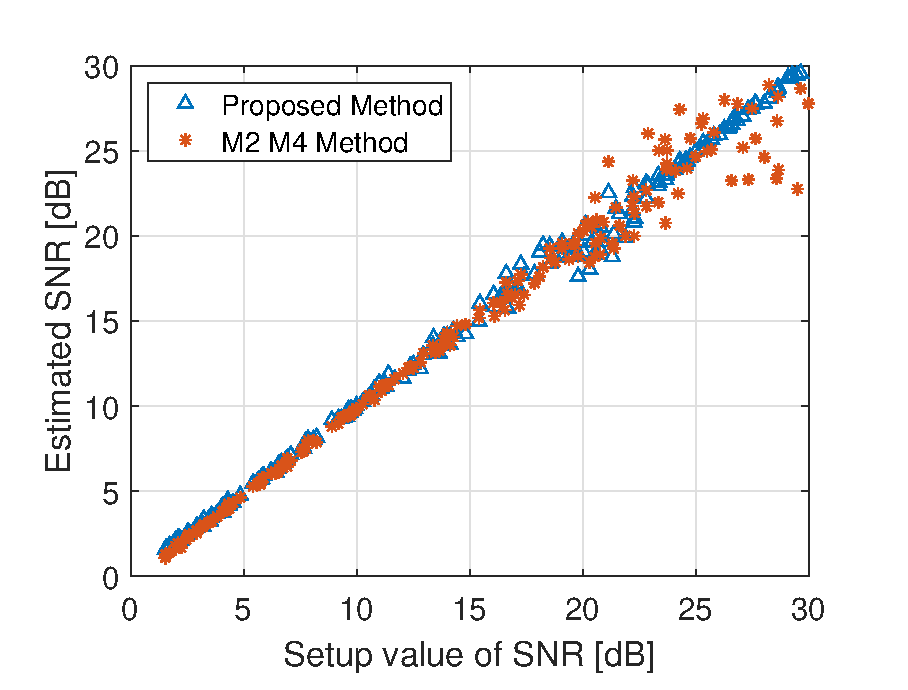
\includegraphics[scale=0.6]{figure/64_regression_compare.eps}}
	\caption{Regression Comparison of proposed method and $M_2 M_4$ method for 64-QAM. }
	\label{fig:regression_compare_64qam}
\end{figure}
\iffalse
\section{Conclusion}
\fi


\chapter{CONCLUSION}
\section{Conclusion}
Optical fiber communication system is becoming very popular for high speed, enormous bandwidth, high security and low cost communication. Due to frequent use of optical fiber communication, it is necessary to monitor SNR (optical signal to noise ratio) for quality management. 

This research work looked for a good estimator for SNR monitoring. For this purpose, a modification in the second and fourth order moment method is performed and an algorithm is developed to solve the problem associated with conventional second and fourth order method. 

MATLAB simulation and investigation proves that proposed method can successfully estimate higher order SNR for 16-QAM less than 1dB monitoring error.

\section{Future works}
16-QAM, 64-QAM, 128-QAM and 256-QAM are some popular quadrature amplitude modulation. In this thesis only a proper solution for 16-QAM and 64-QAM is examined. There are a lot of scope for future development of the conventional second and fourth order method. Our future goal is to develop algorithm for other higher order QAM.

We are hopeful that approaching the same way, we may be successfully develop algorithm for other higher order QAM.



\begin{thebibliography}{9}
	
	\bibitem{OPMTech} 
	Z. Dong, F. N. Khan, Q. Sui, K. Zhong, C. Lu, and A. P. T. Lau,
	\textit{"“Optical performance monitoring: a review of current and future technologies,”"}, 
	IEEE/OSA J. Lightwave Technol. vol. 34, no. 2, pp.525–543, 2016.
	
	\bibitem{deepOSNR} 
	Takahito Tanimura, Takeshi Hoshida, Jens Rasmussen, Makoto Suzuki, Hiroyuki Morikawa.
	\textit{"OSNR monitoring by deep neural networks trained with asynchronously sampled data"}, 
	OptoElectronics and Communications Conference (OECC) 2016.Volume: TuB3-5, July 2016.
	
	\bibitem{inband} 
	M. S. Faruk, Y. Mori, and K. Kikuchi,
	\textit{"In-band estimation of optical signal-to-noise ratio from equalized signals in digital coherent receivers,"}, 
	IEEE Photon. J., vol. 6, no. 1, pp. 1–9, 2014.
	
	\bibitem{eqpsk} 
	D. J. Ives, B. C. Thomsen, R. Maher, and S. J. Savory,
	\textit{"EstimatingOSNR of equalised QPSK signals,"}, 
	Opt. Exp., vol. 19, no. 26, pp.B661–B666, 2011
	
	\bibitem{errorVector} 
	R. Schmogrow, B. Nebendahl, M. Winter, A. Josten, D. Hillerkuss, S. Koenig, J. Meyer, M. Dreschmann, M. Huebner, C. Koos, J. Becker, W. Freude, and J. Leuthold,
	\textit{"Error vector magnitude as a performance measure for advanced modulation formats,"}, 
	IEEE Photonics Technol.Lett., vol. 24, no. 1, pp. 61–63, 2012.
	
	\bibitem{nonlin} 
	Z. Dong, A. P. T. Lau, and C. Lu,
	\textit{"OSNR monitoring for QPSK and 16-QAM systems in presence of fiber nonlinearities for digital coherent receivers,"}, 
	Opt. Exp., vol. 20, no. 17, pp. 19520–19534, 2012.
	
	\bibitem{densityDistributions} 
	A. Yi,L. Yan,H. Liu,L. Jiang,Y. Pan, B. Luo, and W. Pan,
	\textit{"Modulation format identification and OSNR monitoring using density distributions in Stokes axes for digital coherent receivers,"}, 
	Opt. Exp., vol. 27, no. 4, pp. 4471-4479, 2019.
	
	\bibitem{Gaussian} 
	C. Hu, W. Li, H. Zheng, Q. Feng, Q. Zheng and Y. Wang,
	\textit{"A Novel Cost-Effective and Distributed in-Band OSNR Monitoring Method Using Gaussian Process Regression,"}, 
	IEEE Photon. J., vol. 11, no. 4, pp. 1-12, Art no. 7204312, 2019.
	
	\bibitem{non-data-aided} 
	X. Lin, O. Dobre, T. Ngatched, and C. Li,
	\textit{"A non-data-aided OSNR estimation algorithm for coherent optical fiber communication systems employing multilevel constellations,"}, 
	J. Lightw. Technol., vol. 37, no. 15, pp. 3815–3825, 2019.
	
	\bibitem{higher-order} 
	M. Álvarez-Díaz, R. López-Valcarce, C. Mosquera, 
	\textit{"SNR estimation for multilevel constellations using higher-order moments"}, 
	IEEE Trans. Signal Process., vol. 58, no. 3, pp. 1515-1526, 2010.
	
	\bibitem{multilevel} 
	M. S. Faruk and S. J. Savory,
	\textit{"Digital signal processing for coherent transceivers employing multilevel formats,"}, 
	J. Lightw. Technol., vol. 35, no. 5, pp. 1125–1141, 2017.

	\bibitem{limits}
	R.-J. Essiambre, G. Kramer, P. J. Winzer, G. J. Foschini, and B. Goebel,
	\textit{"Capacity limits of optical fiber networks,"}, 
	J. Lightw. Technol., vol. 28, no. 4, pp. 662–701, 2010.
	
	\bibitem{Zhu}
	C. Zhu, A. V. Tran, S. Chen, L. B. Du, C. C. Do, T. Anderson, A. J. Lowery, and E. Skafidas,
	\textit{"Statistical moments-based OSNR monitoring for coherent optical systems,"}, 
	Opt. Exp., vol. 20, no. 16, pp. 17 711–17 721, 2012.
	
	\bibitem{compare}
	David R. Pauluzzi, Beaulieu Beaulieu,
	\textit{"A Comparison of SNR estimation techniques for the AWGN channel,"}, 
	IEEE Transactions on Communications 48(10):1681 - 1691 DOI: 10.1109/26.871393, November, 2000.
		
	\iffalse
	\bibitem{book1} 
	Djafar K. Mynbave, Lowell L. Scheiner. 
	\textit{"Fiber Optic Communication Technology"}, 
	Pearson Education Asia, Singapore,2002.
	
	\bibitem{book2} 
	John M. Senior. 
	\textit{"OPtical Fiber Communication Principles and Practice"}, 
	Prentice Hall of India Private Limited, India, 2004.
	
	\bibitem{book3} 
	D.G Brennan,
	\textit{"Linear Diversity Combining Techniques"}, 
	Proc. IRE, vol.47, pp. 1077-1102, June 1959.
	\fi
	
\end{thebibliography}

\end{document}